\documentclass[11pt]{article}
\usepackage[utf8]{inputenc}
\usepackage[spanish, mexico]{babel}
\usepackage{listings}
\usepackage{breakcites}
\usepackage{dsfont}
\usepackage{hyperref}
\usepackage{amssymb,amsthm,amsmath,latexsym}
\usepackage[margin=1.5cm]{geometry}
\usepackage{natbib}
%\bibliographystyle{stylename}
%\usepackage{fancyhdr}
%\pagestyle{fancy}
\theoremstyle{plain}
\newtheorem{teo}{Teorema}
\newtheorem{prop}[teo]{Proposición}
\newtheorem{defi}[teo]{Definición}
\newtheorem{obs}[teo]{Observación}
\newtheorem{lem}[teo]{Lema}
\newtheorem{cor}[teo]{Corolario}
\usepackage[pdftex]{color,graphicx}
\newcommand{\sgn}{\mathop{\mathrm{sgn}}}
\title{Survey}
\author{Mauricio Gonzalez Soto}
\begin{document}
\nocite{*}
\maketitle
\tableofcontents
\newpage
\section{Introducción}
El problema al cual nos enfrentamos consiste en el aprendizaje de relaciones causales a partir de datos. Los datos que, usualmente, se tienen provienen de fuentes ruidosas por lo que la probabilidad será el lenguaje adecuado para razonar sobre estos datos. Al tratar de averiguar relaciones causales, es común contar con información previa sobre el fenómeno dentro del cual se quiere investigar causalidad, por lo que recurrimos a la estadística bayesiana para el manejo de esta información inicial.\\
\\
La primera parte de este resumen consiste en Redes Bayesianas, que son objetos matemáticos utilizados para representar distribuciones de probabilidad de manera eficiente; además, permiten incorporar conocimiento inicial sobre las variables aleatorias representadas en la red. Debido a que estas redes son de fácil interpretación, es natural definir modelos causales en términos de estas, pues fácilmente nodos y aristas pueden traducirse en términos de objetos y causas.\\
\\
Veremos que al intentar obtener relaciones causales a partir de información proveniente del mundo real necesitamos obtener las entidades que se relacionan entre sí de manera causal, por lo que haremos un repaso de técnicas utilizadas en extracción de relaciones.\\
\\
Por otro lado, en la literatura proveniente de Psicología Computacional y Ciencias Cognitivas, se sabe que los seres humanos obtienen conocimiento causal al encontrarse en situaciones en las cuales deben tomar decisiones de manera secuencial para lograr un objetivo futuro. Se sabe también que el conocimiento causal adquirido es utilizado para mejorar las futuras decisiones tomadas.\\
\\
Finalmente, se discutirá un poco sobre Aprendizaje por Refuerzo, que es un marco teórico para el aprendizaje automático en el cual un \textit{agente} aprende a realizar una tarea a través de experiencia y de interacción con su entorno. Notando que los modelos causales tradicionales requieren de intervenciones y experimentación en el mundo, y que estas intervenciones son una forma de interacción y alteración del mundo, salta a la vista la relación entre Aprendizaje por Refuerzo y aprendizaje causal. Entonces, resulta natural preguntar cómo pueden aprenderse relaciones causales de manera interactiva de modo que el conocimiento causal adquirido permita a un agente tomar mejores decisiones. La pregunta se convierte entonces en cómo obtener e incorporar conocimiento causal en un problema de aprendizaje por refuerzo. Además, uno se pregunta si es posible utilizar este conocimiento causal obtenido al interactuar sobre el mundo para realizar otro tipo de inferencias causales en ciertos dominios de interés.
\section{Causalidad}
\subsection{Intro}
Saber si es posible hablar de relaciones causa-efecto es un tema polémico; los métodos probabilistas tradicionales sólo codifican asociaciones estadísticas, pero la idea
La diferencia entre modelos probabilistas y modelos causales se da cuando es de interés tomar acciones que modifiquen el entorno y no nada más observar los valores de las variables. \\
Según \cite{pearl2014probabilistic}, las dos preguntas fundamentales en Causalidad son:
\begin{itemize}
\item ¿Qué evidencia empírica es necesaria para hacer inferencias válidas sobre relaciones causa-efecto?
\item Dado que estamos dispuestos a aceptar información causal sobre un fenómeno, ¿qué inferencias podemos obtener a partir de esta información, y cómo?
\end{itemize}
En cuanto al segundo punto, Pearl considera que hay tres tipos de preguntas a considerar
\begin{itemize}
\item Predicciones: si sabemos que una persona ingirió alimentos de dudosa procedencia, ¿se enfermará?
\item Intervenciones: si le damos cierto tratamiento a un paciente, ¿mejorará?
\item Contrafactuales: ¿el paciente del punto uno se habría enfermado de todos modos si no hubiera consumido esos alimentos?
\end{itemize}
Pearl argumenta que aunque causalidad suele entenderse como afirmaciones necesarias, estas son hechas en contexto de incertidumbre, por lo que cualquier teoría causal debe estar en términos de probabilidades.
\subsection{Un poco de historia}
Aristóteles definió 4 \textit{causas} para una cosa, una de ellas llamada \textit{causa eficiente} que estaba definida como aquello que hace la cosa.\\
\\
En 1690, el filósofo inglés John Locke propuso como definición de causa “aquello que produce alguna idea simple o compleja”, y lo que es producido lo definió como efecto.\\
\\
\cite{holland1986statistics} resalta la importante diferencia en que Aristóteles hizo énfasis en las causas de una cosa, pero no en el efecto de estas. \\
\\
Fue David Hume quien se considera que hiz una importante contribución, y él definió la causalidad como una relación entre experiencias más que una entre hechos. Argumentó que no es verificable empíricamente que la causa produzca el efecto, sino sólo que el evento llamado \textit{causa} es invariablemente seguido por aquella experiencia llamada \textit{efecto}.\\
\\
Hume definió 3 criterios básicos para causalidad:
\begin{itemize}
\item Contiguidad espacio-temporal: tanto causa y efecto tienen lugar en una entidad común (espacio y tiempo).
\item Sucesión temporal: La causa tiene que preceder temporalmente al efecto. 
\item Conjunción constante: Causa y efecto ocurren juntos, o no ocurren juntos.
\end{itemize}
John Stuart Mill argumentó tajantemente que observación sin experimentos no puede probar causalidad. Mill identificó cuatro métodos generales para la identificación de relaciones causales. 
\subsection{Modelo de Rubin}
El modelo de Rubin parte de una población de \textit{unidades} $U$. En general, estas unidades son los objetos de estudio sobre las cuales actuan las causas. Para hacer más sencilla la descripción del modelo, supondremos que sólo existen dos causas (o niveles de tratamiento) denotadas por $t$ y $c$. Sea $S$ una variable indicadora de la causa a la cual cada unidad $u \in U$ fue expuesta. Además, consideramos dos variables respuesta $Y_t$, $Y_c$. $Y_t(u)$ reoresenta el valor de la respuesta si la unidad $u$ es expuesta a $t$ y análogo para $c$.\\
\\
\begin{defi}
Se define el efecto de la causa $t$ sobre $u$ relativo a la causa $c$ como
\[ Y_t(u) - Y_c(u). \]
Esta expresión se lee de la siguiente manera: $t$ causa el efecto $Y_t(u) - Y_c(u)$ en la unidad $u$ (relativo al control $c$).
\end{defi}
Notemos que es imposible observar simultáneamente el efecto de $t$ y de $c$ sobre una misma unidad $u$ y a esto \cite{holland1986statistics} le llama el Problema Fundamental de la Inferencia Causal. El problema, según explica Holland, radica en la palabra \textit{observar} pues no podemos saber simultáneamente el efecto de exponer a un enfermo en particular a un nuevo tratamiento y al mismo tiempo el efecto de no exponerlo.
\subsection{Modelo de Suppes}
En su libro “Probabilistic Theory of Causality”, (\cite{suppes1970probabilistic}), Patrick Suppes intenta mejorar el análisis de Hume sobre causalidad; en particular, la condición de conjunción constante. Para Suppes, no importa qué sean las causas y los efectos, sino que se puedan expresar como eventos que ocurren bajo ciertas condiciones. Suppes supone que todas las causas necesariamente preceden en el tiempo a sus efectos. Define una causa \textit{prima facie} de un evento como un evento que precede temporalemnte a este y que está asociado de manera positiva con él. Define como una causa espuria a una causa prima facie tal que es condicionalmente independiente del efecto dada otra causa la cual es anterior en el tiempo a la causa prima facie y que está asociada con el evento dada la causa. Una causa genuina es una causa prima facie que no es espuria.
\begin{defi}
Si $r < s$ representan valores de tiempo, se dice que el evento $C_r$ es una causa prima facie del evento $E_s$ si
\[ P(E_s | C_r ) > P(E_s). \]
\end{defi}
\begin{defi}
Un evento $C_r$ se dice que es una causa espuria de un eventi $E_s$ si $C_r$ es una causa prima facie de él y para alguna $q < r < s$ existe un evento $D_q$ tal que 
\[P(E_s | C_r, D_q) = P (E_s | D_q) \]
y además,
\[P(E_s | C_r , D_q) \geq P(E_s | C_r). \]
\end{defi}
Por lo tanto,
\begin{defi}
Para tiempos $r < s$, un evento $C_r$ se dice que es una causa genuina de un evento $E_s$ si $C_r$ es una causa prima facie de $E_s$, pero no es una causa espuria.
\end{defi}
Notemos que Suppes está definiendo la causa de un efecto, más que el efecto de una causa. Además, no hay restricciones a la naturaleza de una causa más allá de que sea un evento que ocurre antes en el tiempo. El modelo de Suppes no puede expresar el efecto de una causa en particular, sólo comportamientos promedio (\cite{holland1986statistics}).\\
\\
En palabras de Holland, la causalidad de Suppes no es más que correlación entre causa y efecto que no puede ser eliminada al parcializar causas legítimas.
\subsection{Modelos Causales en Medicina}
Un caso de aplicación en medicina es determinar que ciertas bacterias causan ciertas enfermedades. Existe un conjunto de postulados planteados por Koch para decidir cuándo un micro-organismo está implicado en una enfermedad. Aunque no existe un planteamiento formal, estos pueden expresarse como (\cite{yerushalmy1959methodology}):
\begin{itemize}
\item El organismo debe estar presente en todos los casos de la enfermedad supuestamente provocada por él.
\item El organismo debe aislarse de los pacientes y cultivarse en estado puro.
\item El organismo cultivado en estado puro debe reproducir el padecimiento. 
\end{itemize}
Estos postulados aseguran que no haya datos que apoyen una hipótesis nula de cero efecto causal. \\
\\
Por otro lado, Hill, quien fue de los primeros en estudiar la asociación entre fumar y cáncer, encontró 9 factores útiles a la hora de decidir que una asociación observada es causal. 
\subsection{Causalidad de Granger en Economía}
La causalidad de Granger se utiliza para series de tiempo, lo cual es de alta importancia en Economía. \cite{holland1986statistics} opina que las ideas esenciales de Granger no están limitadas a series de tiempo y que pueden ser expresadas en términos de variables que actuan sobre unidades de una población.\\
\\
En la teoría de Granger, una variable causa otra variable; es decir ( \cite{holland1986statistics}), las realizaciones de una variable mejoran las predicciones hechas sobre la otra variable. La única parte en la que se utilizan series de tiempo en esta definición es para hablar de valores de las variables definidos hasta un cierto tiempo $t$.\\
\\
Si $X,Y,Z$ son variables aleatorias definidas sobre cierta población, se dice que $X$ no es una causa de Granger de $Y$ si $X$ y $Y$ son condicionalmente independientes dado $Z$. Entonces, $X$ es una causa de Granger de $Y$ si distintos valores de $X$ llevan a distintas distribuciones predictivas de $Y$ dados $X$ y $Z$; esto es, $X$ ayuda a predecir $Y$ aun cuando $Z$ es tomada en cuenta. La no-causalidad de Granger es parecida a las causas espurias de Suppes pues ambas consideran que no se pueda predecir un evento dada cierta información.\\
\\
En opinión de Holland, la causalidad de Granger falla de la misma manera que la de Suppes, pues a la luz de nueva información una causa Granger puede dejar de serlo.
\subsection{Modelos Causales en Ciencias Sociales}
\subsection{Aprendizaje de Modelos Causales a partir de datos}
En los métodos de estado del arte de Modelos Causales Funcionales suele hacerse los siguientes supuestos (\cite{goudet2017learning}):
\begin{itemize}
\item Suficiencia Causal (CSA)
\item Propiedad Markoviana (CMA)
\item Independencias Condicionales
\item Fiabilidad causal (CFA)
\end{itemize}
\subsubsection{Aprender el CPDAG}
Existen tres familias de métodos para extraer el grafo: métodos de restricciones, métodos de score y métodos híbridos.\\
\\
Los métodos basados en restricciones explotan las independencias condicionaes para identificar todas las v-estructuras. El algoritmo más conocido es el Algoritmo PC (\cite{spirtes2000causation}). El algoritmo PC primero construye un esqueleto basado en independencias condicionales; luego, identifica las v-estructuras y posteriormente orienta las aristas. El algoritmo FCI (\cite{spirtes1999algorithm}) extiende el algoritmo PC al relajar la suficiencia causal e incorporar variables latentes. El algoritmo RFCI de \cite{colombo2012learning} es más rápido que FCI y maneja datos de alta dimensionalidad. La debilidad de estos métodos, según \cite{goudet2017learning} es que dependen demasiado en pruebas de independencia, que dependen a su vez de la cantidad disponible de datos.\\
\\
Los métodos basados en score exploran el espacio de CPDAG's y minimizan un score global. La exploración se realiza en términos de operaciones sobre grafos, por ejemplo añadir o remover aristas. El algoritmo Greedy Equivalent Search (GES) de \cite{chickering2002optimal} encuentra la estructura óptima en términos del BIC.\\
\\
Los métodos híbridos combinan las técnicas anteriores. Por ejemplo el Max-Min Hill Climbing Algorithm de \cite{tsamardinos2006max} primero construye un esqueleto utilizando pruebas de independencia condicional, y luego le da orientación a las aristas utilizando un método greedy sobre un score bayesiano.
\subsubsection{Explotando la asimetría entre causa y efecto}
Los métodos anteriores no toman en cuenta la asimetría entre causas y efectos. La intuición detrás (\cite{goudet2017learning}) está dada por el siguiente ejemplo: Si consideramos el modelo causal funcional $Y=X+U$, entonces los métodos anteriores basados en grafos no pueden darle orientación a la arista $X - Y$, pues tanto $X \rightarrow Y$ como $Y \rightarrow X$ son Markov equivalentes.\\
\\
\cite{stegle2010probabilistic} infiere la dirección causal al construir dos modelos Bayesianos generativos: uno para $X \rightarrow Y$ y otro para $Y \rightarrow X$. La dirección causal es determinada a partir del modelo generativo que mejor ajuste a los datos. Otros métodos, como el propuesto por \cite{sgouritsa2015inference} se basan en que si $X \rightarrow Y$, entonces la probabilidad marginal de la causa $P(X)$ es independiente del mecanismo causal $P(X | Y)$; por lo tanto, estimar $P(Y | X)$ a partir de $P(X)$ no debería poderse, pero estimar $P(X | Y)$ a partir de $P(Y)$ sí debería ser posible.
\subsubsection{Como problema de Aprendizaje}
Inspirados en los concursos de Kaggle de \cite{Guyon2013}, \cite{lopez2015towards} plantean el problema de inferencia causal como un problema de clasificación de medidas de probabilidad. Los datos provistos por el concurso son 16,200 parejas de variables $(X_i,Y_i)$. Cada par consta de una realización $(x_i,y_i)$ y una etiqueta $l_i$ que indica el valor de la verdadera relación causal; es decir, $l_i$ indica uno de los siguientes casos: $X \rightarrow Y,$ $Y \rightarrow X$, $X_i \perp Y_i$, $X \leftrightarrow Y$.\\
\\
Notemos que este método tiene como punto débil que depende de la representatividad de la muestra de entrenamiento y que supone la existencia de una distribución madre
\subsubsection{Modelos Causales Funcionales Neuronales}
\cite{goudet2017learning} proponen un esquema que consiste en tres pasos: primero, identificar el esqueleto según propiedades de independencia estándar; luego, orientar las aristas utilizando métodos bivariados estándar y finalmente hacer una optimización sobre todo el grafo examinando relaciones locales. Este último paso se realiza al aprender estos modelos locales como redes neuronales generativas; es decir, se modela la distribución $P(X | X_{Pa_i}, U_i)$ de un nodo condicional en sus padres (causas) con una red neuronal.\\
\\
Formalmente, se modela cada ecuación
\[X_i = f_i (X_{Pa_i},U_i) \]
como una red neuronal generativa global, en la cual cada función $f_i$ es modelada por una red neuronal generativa con una capa oculta.\\
\\
Encontrar un modelo causal de este tipo requiere llevar a cabo dos tareas: estimar la estructura (el grafo) de los padres de cada variable, y las redes neuronales $f$
\subsection{Correlación y causalidad}
Dos variables aleatorias $X$,$Y$ pueden estar correlacionadas en distintos casos; por ejemplo, si $X$ causa $Y$, o si tanto $X$ como $Y$ son causadas por otra variable desconocida $V$. Si e conoce la existencia de $V$ y además podemos observarla. 
\section{Modelos gráficos causales}
Sabemos que en una red bayesiana los arcos, aunque dirigidos, no necesariamente tienen una interpretación directa, lo único que importa es que el grafo capture adecuadamente las relaciones de dependencia entre variables aleatorias. Nos gustaría que fuera el caso que $X \to Y$ significara $X$ \textit{causa} Y. Resulta que existe una familia de modelos causales en los cuales se \textit{interviene} en el mundo. La idea clave es utilizar \textit{intervenciones ideales}, las cuales se denotan $do(Z=z)$ que significa forzar a la variable aleatoria $Z$ a tomar el valor $z$, denotado de manera simple como $do(z)$. Esta operación corresponde al caso en que un agente directamente modificó el estado del mundo y no sólo observó los valores de este de manera pasiva; por esta razón es muy importante tener en mente que es distinto $P(Y | do(z), X=x)$ que $P(Y | Z=z, X=x)$. Las preguntas causales de interés son planteadas de la forma $P(X | do(z))$ y son llamadas \textit{quries intervencionales}. Este tipo de intervenciones surgen de manera natural en muchos problemas; por ejemplo, “si el paciente recibe este tratamiento, cuál es la probabilidad de sobrevivir la enfermedad” puede ser planteada como $P(sobreivir | do(tratamiento))$.\\
\\
Formalmente, un modelo gráfico causal (\cite{koller2009probabilistic}, \cite{pearl2014causality}) tiene la misma forma que una red Bayesiana; es decir, consiste en una red acíclica dirigida que codifica una distribución entre un conjunto de variables aleatorias. La diferencia radica en la interpretación de las flechas, pues cada variable aleatoria está gobernada por un modelo causal en función de sus padres en el grafo. Una intervención consiste en forzar uno de los nodos a tomar un valor con probabilidad 1 y a recortar todas las flechas que entran en ese nodo.\\
\\
Es importante que se cumpla que si dos variables están correlacionadas, entonces una es padre causal de la otra y que no falten padres causales de ninguna variable.\\
\\
Para poder contestar pregunta acerca de intervenciones, se necesita introducir el concepto de \textit{grafo mutilado}
\begin{defi}
Sea $\mathcal{B}$ una red sobre un conjunto de variables aleatorias y sea $Z_1=z_1,...,Z_k=z_k$ una instanciación de estas variables denotada por $\mathbf{Z}=\mathbf{z}$ . Se define el grafo mutilado $\mathcal{B}_{\mathbf{Z}=\mathbf{z}}$ como:
\begin{itemize}
\item Cada nodo $Z_i \in \mathbf{Z}$ no tiene padres en $\mathcal{B}_{\mathbf{Z}=\mathbf{z}}$
\item El modelo local de probabilidad condicional para $Z_i \in \mathbf{Z}$ es tal que asignal probabilidad uno al valor $z_i$ y cero a cualquier otro valor.
\item No se altera ningún otro nodo $X_i \notin \mathbf{Z}$
\end{itemize}
\end{defi}
Entonces, utilizando este concepto, tenemos que para un modelo causal $\mathbf{C}$ una intervención $P_{\mathcal{C}}(Y|do(z)$ es realmente una \textit{querie} probabilista estándar, pero en el grafo mutilado dado por $\mathcal{C}_{Z=z}$; es decir
\[ P_{\mathcal{C}}(Y|do(z),x) = P_{\mathcal{C}_{Z=z}}(Y|x).  \] 
\subsection{Identificabilidad de modelos}
Aun a pesar de desconocer la totalidad de las variables latentes causales, existen casos en los que es posible responder a preguntas causales en modelos que involucran variables latentes utilizando sólo variables observadas; este es el caso de los modelos identificables. Existen formas de simplificar queries intervencionales y convertirlas en queries que sólo requieren de datos observacionales pues existen equivalencias entre unas y otras bajo ciertas condiciones.\\
\\
\cite{peters2012identifiability} exploran las condiciones para obtener identificabilidad en modelos causales funcionales. 
\subsection{Aprendizaje de modelos gráficos causales}
Según \cite{koller2009probabilistic}, el problema de aprender un modelo causal a partir de datos puede dividirse en varios ejes:
\begin{itemize}
\item En primer lugar, definir qué se entiende por un modelo causal, pues si estamos trabajando con modelos gráficos causales entonces el problema se convierte en aprender redes bayesianas, pero con la diferencia de la interpretación que se da a las flechas; por otro lado, en modelos causales funcionales se tienen parametrizaciones mucho más complejas para las variables de respuesta, por lo que se necesitan modelos más complejos como el modelo neuronal presentado anteriormente.
\item Un segundo eje es determinar si ya se conoce la estructura y sólo se necesita aprender la parametrización, o si también debe ser aprendida la parametrización.
\item En tercer lugar, es el tipo de datos: observados o intervencionales. Datos observados son aquellos que provienen de alguna distribución generadora y datos intervencionales es en aquellos en los que se intervino el modelo y se observó la respuesta de este. Los datos intervencionales son difíciles de obtener en la práctica, o incluso pudieran ser inmorales o ilegales.
\item Finalmente, cómo tratar los factores de confusión (confounding factors). Uno puede suponer que simplemente no existen y en estos casos el problema se vuelve relativamente sencillo.
\end{itemize}
\subsubsection{Aprender sin factores de confusión}
El problema de aprender modelos gráficos causales sin factores de confusión es esencialmente el mismo que aprender redes bayesianas (\cite{koller2009probabilistic}), pero hay que hacer algunas suposiciones importantes, pues existen siempre varios DAG's que representen la misma distribución, pero que tendrían distintas interpretaciones causales. Una de las suposiciones necesarias para poder aprender modelos causales a través de datos observacionales es la llamada Propiedad Causal de Markov, que es un análogo a la Propiedad de Markov para redes Bayesianas; y su formulación es la siguiente (\cite{koller2009probabilistic}): \textit{cada variable es condicionalmente independiente de sus no-efectos dadas sus causas directas.} El otro supuesto necesario es que las únicas independencias condicionales sean aquellas que surgen de la d-separación en el grafo causal correspondiente (\textit{faithfulness}).\\
\\
Aun con estas suposiciones, lo más que puede aprenderse es una clase de equivalencias para el grafo causal y para llevar esto a cabo existen dos familias de métodos: basados en restricciones y basados en score y son los mismos que se utilizan para aprender el CPDAG en modelos causales funcionales.
\subsubsection{Aprender de datos intervencionales}
En el caso en que se tienen datos provenientes de intervenciones, lo cual es lo más común en el contexto de experimentos científicos. Se utilizan métodos basados en score para aprender de este tipo de datos.
\subsubsection{Aprender con variables latentes}
En el caso en el que suponemos que existen variables latentes, estamos pensando que los datos fueron generados por una distribución que es \textit{parecida}, o parcial, a la verdadera. De nuevo, existen familias de métodos basadas en restricciones y métodos basados en scores.
\subsection{Redes Bayesianas causales: aplicación en genética}
\cite{su2013using} intentan aprender la estructura de las relaciones entre un conjunto de variables relacionadas a un estudio de cáncer (\cite{karagas1998design},\cite{karagas2004incidence}). Específicamente, los autores analizan sólo 11 variables relacionadas a un solo gen. Identifican relaciones interesantes, como por ejemplo la variable “fumador” como padre causal de la variable “cancer”, aunque no apareció relación entre la variable cancer y un gen que se sabe está relacionado con el cáncer, pero esto se debe a la manera en la que fueron seleccionados los pacientes.
\section{Modelos causales funcionales y ecuaciones estructurales}
En otras áreas, como las ingenierías y la física, las relaciones causales se expresan como relaciones funcionales determinísticas en donde cualquier componente aleatorio se introduce en términos de variables no observadas. Esto corresponde (\cite{pearl2009causality}) a la noción Laplaciana de lo aleatorio. En este contexto, un modelo causal funcional consiste en un conjunto de ecuaciones de la forma
\[ X_i = f_i (X_{Pa_i},U_i), \textrm{  } i=1,...n\]
donde $Pa_i$ corresponde al conjunto de variables que directamente determinan a la variable con índice $i$ y donde $U_i$ representa cualquier error de medición o de aspectos no observados.\\
\\
Dado un modelo causal de esta forma, podemos obtener un diagrama de la siguiente manera: para cada variable pintamos un nodo, y desde cada elemento de $Pa_i$ dibujamos una flecha hacia el nodo que corresponde a $X_i$. A este diagrama se le llama \textit{diagrama causal}. Si cumple que el diagrama es acíclico, se le conoce como semi-Markoviano. Si, además de ser acíclico, los términos de error son independientes entonces se dice que es Markoviano. El siguiente Teorema muestra la conexión entre el diagrama causal y la distribución de probabilidad asociada. 
\begin{teo}
Todo modelo causal Markoviano induce una distribución $P(X_1,...,X_n)$ que satisface que cada variable $X_i$ es independiente de todos sus no-descendientes dado sus padres $Pa_i$.
\end{teo}
Sabemos que dos DAG's que tienen el mismo esqueleto y las mismas v-estructuras son equivalentes, y a la clase de equivalencia le llamaremos CPDAG (\cite{goudet2017learning})
\subsection{Intervenciones y efectos causales en modelos funcionales}
Los modelos funcionales causales proveen una manera de estimar cómo cambiaría la distribución en respuesta a cambios externos. Lo que se hace en estos modelos es representar las intervenciones como alteraciones a un conjunto de funciones. El efecto total de la intervención se calcularía modificando las ecuaciones correspondientes y con este nuevo modelo calcular las nuevas probabilidades. Denotamos una intervención como $do(X=x)$. Se dice que una variable $X_i$ es causa directa de $X_j$ si
\[ P_{X_j | Do(X_i = x_i} \neq P_{X_j | do(X_i = x')} \]
\subsection{Contrafactuales en modelos funcionales}

\section{Extracción de relaciones causales a partir de texto}
\subsection{Extracción basada en patrones gramaticales}
\cite{khoo2000extracting} desarrollan un método que permite identificar y extrar relaciones causa-efecto que se encuentra expresada de manera explícita en \textit{abstracts} de artículos médicos. Los autores deciden utilizar el dominio médico pues al ser importantes las relaciones causales es más probable que estas aparezcan explícitamente. Los autores primero identifican los \textit{marcadores lingüísticos} y con esto construyen un conjunto de \textit{patrones causales}. Además, cada oración es pasada por un \textit{parse tree} el cual genera una representación de la estructura sintáctica de la oración.\\
\\
Como ejemplo, consideremos la oración \textit{“Paclitaxel was well tolerated and resulted in a significant clinical response in this patient”}. Después de la creación del árbol sintáctico y del patrón gramatical, se obtiene que la causa presente en la oración es \textit{paclitaxel} y el efecto es \textit{a significant clinical response in this patient}.\\
\\
Analizando 200 abstracts que provienen de 4 áreas médicas (depresión, esquizofrenía, enfermedades cardiacas y SIDA), construyen los patrones causales. El proceso de extracción de información consiste en hacer un \textit{match} entre los patrones causales y el arbol sintáctico. Al aplicar los patrones causales obtenidos a un nuevo conjunto de abstracts, obtienen un 51 por ciento de accuracy al extraer causas y un 58 por ciento de accuracy al extraer efectos.\\
\\
\cite{girju2002text} presentan un método semi-automático para la detección de patrones causales en texto, es semi-automático pues los patrones son descubiertos de manera automática, pero la validación no lo es. El algoritmo de detección de patrones léxico-sintácticos que  se refieren a causalidad consiste en dos partes. La primera parte descubre patrones léxico sintácticos que pueden expresar relaciones causales, y la segunda valida estos patrones según restricciones semánticas. Se enfocan en encontrar patrones de la forma (frase verbo causal frase) donde el verbo es un verbo causal simple en los cuales el verbo se refiere únicamente a la causa; por ejemplo, \textit{Temblores generan tsunamis}. Como las frases obtenidas pueden ser muy largas, pueden aportar información no deseada. Para resolver esto \cite{girju2003automatic} utiliza WordNet para reducir el tamaño de las frases obtenidas.\\
\\
\cite{sanchez2004acquiring} desarrollan un sistema para la adquisición de conocimiento causal a partir de texto. El sistema propuesto identifica oraciones que especifican de manera explícita relaciones causales y extrae de ellas los patrones causales. El sistema incorpora información gramatical tal como conectores, conjunciones, disjunciones y negaciones y codifican todo esto en redes bayesianas.\\
\\
Para la detección de patrones causales, los autores se enfocan en trabajar con oraciones en las cuales ambos \textit{eventos} aparezcan como frases (noun phrases, ¿traducción?). Un ejemplo de patrones causales identificados por el sistema es \textit{“Anemia are caused by excessive hemolysis”}.
\\
Para la construcción de las redes, se toma como input un texto \textit{tokenizado}, etiquetado con \textit{part-of-speech tagging} y \textit{parsed} para encontrar expresiones verbales. Posteriormente, el sistema estima las probabilidades condicionales de los efectos dadas las causas mediante el conteo de frecuencias de eventos similares.\\
\\
Para la evaluación, hicieron una evaluación subjetiva que consistió en comparar la estructura de la red generada por el sistema y la estructura creada manualmente al observar los patrones causales en el texto. Se analizaron 7 textos y en general se encontró un empate entre las redes con una precisión de 60 por ciento, pero sin ningún valor de Recall, por lo que no es fácil interpretar sus resultados. Según \cite{bojduj2009extraction}, una de las razones por las cuales se ubtuvo baja precisión es que basar los nodos en las frecuencias no es una buena idea, pues la cantidad de texto disponible en general es tan grande que estas frecuencias no pueden ser representativas.\\
\\
\cite{bojduj2009extraction} menciona que muchos de estos métodos están más enfocados en cómo extraer las relaciones que en cómo usarlas. Es importante no sólo poder concluir que dos términos están relacionados causamente, sino cómo.
\subsection{Extracción basada en patrones de co-ocurrencias}
En vez de utilizar patrones gramaticales, \cite{saito2007extraction} y \cite{perrin2008global} analizan la co-ocurrencia de términos estadísticos para construir redes a partir de texto. Ellos definen un “statistical term” como \textit{“Statistical terms are expression of the measurements of statistics to watch the movements of phenomena; birth rates, public approval rating of the Cabinet and so on.”}; es decir, un término que sea importante a un sistema. El enfoque de su trabajo es construir redes causales entre los statistical terms. Lo que hacen es primero extraer relaciones de co-ocurrencia entre términos estadísticos y posteriormente extraer relaciones causales entre ellos. Los autores se enfocan en texto japonés, el cual cumple que tiene ciertos patrones en los sufijos utilizados, y estos patrones son utilizados al extraer los términos estadísticos. Luegom estos términos son clasificados según su nivel de abstracción. Posteriormente, construyen una red de términos estadísticos al considerar a dos de ellos co-ocurrentes si aparecen juntos en un párrafo. Se remueven los términos que son co-ocurrentes con muchos otros términos.\\
\\
Los autores evaluan de manera separada cada una de las etapas: extracción de términos, clasificación de términos, la construcción de redes y la clasificación de redes.
\\
La mayor desventaja de esto es que la dirección de la relación causal no puede ser inferida de la co-ocurrencia.\\
\\
Por otro lado, \cite{sakai2008cause} extrajeron términos de artículos financieros (en japonés) y luego considerarón que estos términos afectaban el desempeño de los negocios basados en co-ocurrencias con expresiones clave como “es bueno”. Su definición de causalidad depende de las expresiones clave.
\subsection{Modelos Gráficos para extracción de relaciones}
A partir de un artículo que trata específicamente sobre una entidad claramente indentificable (la biografía de Benito Juarez por ejemplo) \cite{yu2010jointly} intentan identificar entidades y descubrir relaciones semánticas entre ellas. Resulta evidente que en el documento aparecerán otras entidades, pero se hace el supuesto de que no están relacionadas entre sí. En este trabajo, todas las clases entidades están pre-definidas así como las relaciones; esto es, se sabe que en el documento aparecerán años, lugares, países y que una entidad de tipo persona habrá nacido en un país en cierto año. Para formular el problema, se tiene $\mathbf{x} = \{ x_1,...,x_N \}$ una sucesión observada de \textit{tokens}. Denotamos como $s_p$ la entidad principal. Sea $ \mathbf{s}=\{ s_1,...,s_L\}$ una segmentación en la cual cada $s_i$ es una tripleta $\{ \alpha_i, \beta_i,y_i \}$ con $\alpha_i$ es una posición inicial, $\beta_i$ posición final y $y_i$ una etiqueta asignada.\\
\\
Sea $r_{pn}$ la asignación de relaciones entre la principal $s_p$ y un candidato a entidad secundaria $s_n$ y sea $\mathbf{r}$ el conjunto de asignación de relaciones para la $\mathbf{x}$. Dada una observación $\mathbf{x}$, queremos encontrar $\mathbf{y}^\ast$ tal que
\[ \mathbf{y}^\ast = \textrm{ arg max }_y p(\mathbf{y}| \mathbf{x})\]
donde $\mathbf{y}=\{ \mathbf{r},\mathbf{s} \}$.\\
\\
Se define una distribución condicional conjunta para $\mathbf{s},\mathbf{x},\mathbf{r}$ en un modelo grafico no dirigido $\mathcal{G}$ tal que se pueden dividir los factores de $\mathcal{G}$ en tres grupos: $\phi^S$, $\phi^R$, $\phi^\nabla$, que son el potencial de segmentación, el potencial de relaciones, y el potencial conjunto de segmentación-relación. \\
\\
Por el Teorema de Hammersley-Clifford, la condicional conjunta $P(\mathbf{y} | \mathbf{x})$ se factoriza como
\[ P(\mathbf{y} | \mathbf{x}) = \frac{1}{Z(\mathbf{x})} \prod_{C_S} \phi^S (i,\mathbf{s},\mathbf{x}) \prod_{C_R}\phi^R(r_{pm},r_{pn},\mathbf{r}) \prod_{C_\nabla} \phi^\nabla(s_p,s_j,\mathbf{r}) \]
Se hace el supuesto de que las funciones potencial se factorizan según un conjunto de atributos y un conjunto de pesos correspondientes.\\
\\
Incorporando estos features, tenemos que 
\[P(\mathbf{y} | \mathbf{x}) = \frac{1}{Z(\mathbf{x})} \exp \left( \sum_{i=1}^{|s|} \sum_{k=1}^K \lambda_k g_k(i,s,x) + \sum_{m,n}^M \sum_{w=1}^W \mu_w q_w (r_{pm},r_{pn},r) + \sum_{j=1}^L \sum_{t=1}^T  \nu_t h_t(s_p,s_j,r) \right) \]
\\
Dada una muestra $\mathcal{D}= (\mathbf{x}_i, \mathbf{y}_i)_{i=1}^N$ queremos estimar los parámetros $(\lambda_k,\mu_w,\nu_t)$.\\
\\
La log-verosimilitud regularizada es
\[ \mathcal{L} = \log [\Phi(r,s,x)] - \log [Z(x)] - \sum_{k=1}^K \frac{\lambda_k^2}{2 \sigma_\lambda^2} - \sum_{w=1}^W \frac{\mu_w^2}{2 \sigma_w^2} - \sum_{t=1}^T \frac{\nu_t^2}{2 \sigma_\nu^2} \]
Donde,
\[ \Phi(r,s,x) = \exp (\sum_{i=1}^{|s|} \sum_{k=1}^K \lambda_k g_k(i,s,x) + \sum_{m,n}^M \sum_{w=1}^W \mu_w q_w (r_{pm},r_{pn},r) + \sum_{j=1}^L \sum_{t=1}^T  \nu_t h_t(s_p,s_j,r)) \]
Tenemos que $\mathcal{L}$ es concava por lo que es fácil maximizarla.\\
\\
Para calcular la Asignacion Más Probable, hayue encontrar
\[ \mathbf{y}^\ast = \textrm{ arg max }_y p(\mathbf{y}| \mathbf{x})\]
La cual no se puede resolver de manera exacta, se necesitan métodos aproximados. El algoritmo que se propone en el artículo se llama Collective Iterative Classification y la idea detrás de este es decodificar las variables ocultas objetivo basados en asignar etiquetas a las variables muestreadas. Esto se hace mediante un proceso iterativo de dos pasos; primero, en una etapa de bootstrapping se predice una etiqueta inicial para una $x_i$ dado el modelo ya entrenado. Luego, en la segunda etapa, conocida como clasificación iterativa, se re-estima la asignación a $x_i$ varias veces, tomándolas a partir de la asignación inicial.\\
\\
Los autores prueban su algoritmo con datos provenientes de Wikipedia: sus datos consisten en 441 páginas de Wikipedia. De estos datos, fueron etiquetados a mano 7740 entidades en 8 categorías. Además, se extrajeron 4700 relaciones de las cuales las más frecuentes fueron trabajo, visió, nació, miembro de, nació en día.\\
\\
El modelo superó los existentes tomando como medida de calidad la medida F. 
\section{Métodos Estadísticos Para Extracción de Relaciones Causales}
\subsection{Statistical Relational Learning}
En el contexto de inferencia causal, se estudian las interacciones entre variables que puedan causar efectos en la otra. Para esto, es necesario identificar los objetos y las relaciones entre ellos. Para esto, el área de Statistical Relational Learning ofrece una serie de métodos que modelan dependencias entre entidades relacionales. En esta sección veremos distintas técnicas existentes en esta área y sus aplicaciones a inferencia causal.\\
\\
Un dominio de interés consiste en objetos (entidades), sus atributos, y las relaciones entre sí de los objetos. El modelo DAPER de \cite{heckerman2004probabilistic} consiste en clases de entidades, clases de relaciones, clases de atributos y clases arco.
\subsubsection{Aplicación de Campos Aleatorios Condicionales a Extraccion de informacion}
\cite{ramani2005consolidating} analizaron 753,459 abstracts de journals médicos, de los cuales extrajeron 6580 interacciones entre 3,737 proteínas. Para ello, utilizaron un algoritmo de tres etapas: la primera etapa, consiste en identificar nombres de proteínas mediante un clasificador basado en Conditional Random Fields; la segunda, identificar interacciones a través de co-ocurrencias; posteriormente, filtrar estas interacciones con un clasificador Bayesiano para obtener interacciones válidas. Con esto, se obtiene una red que consiste en 31609 interacciones entre 7748 proteínas\\
\\
Para la etapa de identificación de nombres, se utilizó un Conditional Random field, cuyo desempeño fue evaluado en un conjunto de 200 abstracts médicos etiquetados y en 750 abstracts etiquetados a mano. Para extraer los nombres de proteínas, se utilizó este clasificador en el conjunto de 753,459 abstracts de Medline que contuvieran la palabra “human”.\\
\\
Para obtener las interacciones, se midió la co-citación entre los nombres de proteínas y luego se enriquecieron estos pares con interacciones físicas (reales) entre proteínas utilizando un filtro Bayesiano. Primero, se contó el número de veces que en un abstract aparece un par de proteínas, y con eso se calculó la probabilidad de co-citación. Con esto se obtienen 15,000 interacciones, pero se pueden dar co-citaciones por otras razones además de las relaciones reales, se aplicó un filtro bayesiano que mide la verosimilitud de los abstracts que citan un par de proteínas para discutir sus interacciones reales. El clasificador asigna un \textit{score} a cada uno de los abstracts que citan esas proteínas. Utilizando un umbral de score, se obtienen 6,580 interacciones entre 3,737 proteínas.\\
\\
Al combinar estas interacciones con otras 26,280 interacciones provenientes de otras fuentes, se obtiene el total mencionado.\\
\\
Por otro lado, \cite{culotta2006integrating} plantean el problema de extracción de relaciones como un problema de etiquetado de secuencias, algo similar a lo realizado por \cite{yu2010jointly}.   \cite{culotta2006integrating} definen un modelo de la forma
\[ P_{\Lambda} ( y | x ) =\frac{1}{Z} \prod_{c \in C} \varphi_c ( y_c , x_c, \Lambda ),\]
donde las $\varphi$ son potenciales parametrizados por $\Lambda$.\\
\\
Los autores tomaron 1,127 párrafos de 271 artículos biográficos de Wikipedia y etiquetaron 4,701 instancias de relaciones. Para identificar a las entidades importantes dentro de un artículo, utilizaron el hecho de que estas suelen tener un \textit{hyperlink}
\subsubsection{Aplicación de RMN's a Extraccion de informacion}
\cite{bunescu2007statistical} utilizan Relational Markov Networks para mejorar el desempeño de los CRF's en el problema de identificar nombres de proteínas en abstracts de journals médicos. \\
\\
La técnica que se propone es que dada una colección de documentos $D$, asociemos a dada documento $d \in D$ un conjunto de entidades $d.E$. Cada entidad$e \in d.E$ queda caracterizada por un conjunto de atributos booleanos $e.F$. A cada documento se le asocia un grafo de factores, el cual es un grafo bipartita que contiene dos tipos de nodos: nodos variables, que corresponden a las etiquetas de todas las entidades candidato en el documento y nodos potenciales, que modelan las correlaciones entre dos o más atributos. Para cada correlación posible,  un nodo potencial es crreado tal que está ligado a todos los nodos variables involucrados.\\
\\
Prueban su algoritmo en dos conjuntos de datos previamente etiquetados a mano. El primer conjunto consiste en 200 abstracts y el segundo en 225. Ambos conjuntos de datos fueron previamente etiquetados a mano, además de etiquetados para POS. En ambos conjuntos de datos, existe una mejora ligera respecto a los CRF's en términos de la medida F.

\subsubsection{Aprendizaje de Modelos Causales a partir de Datos Relacionales}
\cite{maier2013reasoning} definen la \textit{abstract ground graph} (AGG) y se desarrolla la noción de d-separación relacional. A partir de estas nociones teóricas, \cite{maier2013sound} extienden el algoritmo PC, el cual identifica todas las posibles orientaciones de dependencias causales, a datos relacionales. Utilizando la d-separación relacional, introducen restricciones que orienta dependencias bivariadas hasta en un 72$\%$ más. Se prueba teóricamente que con esta nueva regla, además de extensiones a datos relacionales del algoritmo PC, se obtiene un método \textit{sound and complete} para la extracción de relaciones causales. Este algoritmo nuevo se llama RCD (relational causal discovery).\\
\\
\cite{lee2016learning} notan que la demostración de \cite{maier2013reasoning} requiere que la AGG sea un DAG quie represente exactamente todas las flechas que aaparecerían en todas las posibles ground graphs, y en un trabajo anterior (\cite{lee2015lifted}) habían notado que existen casos en los cuales la d-separación de la AGG no captura las independencias condicionales que se cumplen en el modelo relacional causal. En su artículo, proponen un algoritmo basado en condiciones más débiles llamado RCD-light.

\subsection{Inferencia Bayesiana No Paramétrica}
La rama no-paramétrica de la inferencia bayesiana puede considerarse como una extensión a espacios infinito-dimensionales de la inferencia bayesiana clásica. Esto permite tener modelos que permiten capturar una complejidad mucho mayor en los datos. El objeto principal de la inferencia bayesiana no paramétrica es el Proceso Dirichlet, que es una extensión a espacios infinito-dimensionales de la distribución Dirichlet clásica.
\subsubsection{Proceso Dirichlet}
\begin{defi}
Sea $H$ una medida finita definida sobre un espacio $\mathcal{X}$ y $\alpha \in \mathbb{R}$. Una medida aleatoria $G$ sobre $\mathcal{X}$ se dice que es un Proceso Dirichlet de parámetros $(\alpha,H)$ si para cada partición finita medible $\{ A_1 , ..., A_k \}$ de $\mathcal{X}$ se tiene que la distribución conjunta de $(G(A_1),...,G(A_k))$ es Dirichlet de parámetros $(\alpha H(A_1),...,\alpha H(B_k))$. A la medida $H$ se le conoce como medida base y a $\alpha$ se le conoce como parámetro de concentración. Se denota como
\[ G \sim \textrm{ DP}(\alpha,H).\]
\end{defi}
Los parámetors $H$ y $\alpha$ juegan roles intuitivos en la definición. La medida base se puede entender, básicamente, como la \textit{media} del Proceso; es decir, para cada conjunto medible $A \subseteq \mathcal{X}$ se tiene que $\mathbb{E}[G(A)]=H(A)$. Por otro lado, el parámetro de concentración es un tipo de \textit{varianza inversa}, pues $V[G(A)]=H(A)(1-H(A))/(\alpha+1)$. Es decir, mientras más grande sea $\alpha$, entonces menor es la varianza y el DP tenderá a concentrarse más en torno a $H$.\\
\subsubsection{Distribución Predictiva y urnas de Blackwell-McQueen}
Consideremos $G \sim \textrm{ DP}(\alpha,H)$ y $\theta_1,... \sim G$. Como $\theta_{n+1} | G, \theta_1,...,\theta_n \sim G$, entonces para $A \subseteq \mathcal{X}$ tenemos que
\begin{eqnarray*}
P(\theta_{n+1} \in A | \theta_1,...,\theta_n ) &=& \mathbb{E}[G(A) | \theta_1,...,\theta_n]\\
                                                                    &=& \frac{1}{\alpha + n} \left(\alpha H(A) + \sum_{i=1}^n \delta_{\theta_i}(A) \right)
\end{eqnarray*}
Por lo tanto, marginalizando $G$, vemos que la distribución posterior base dados $\theta_1,...,\theta_n$ es la distribución predictiva de $\theta_{n+1}$.
\[ \theta_{n+1} | \theta_1,...,\theta_n \sim \frac{1}{\alpha + n} \left( \alpha H + \sum^n \delta_{\theta_i} \right) \]
La secuencia de distribuciones predictivas para $\theta_1, \theta_2,...$ se conoce como el esquema de urnas de Blackwell-McQueen; la interpretación es la siguiente: cada valor en $\mathcal{X}$ es un color, y cada realización $\theta \sim G$ son pelotas y el valor obtenido es el color de la pelota. Además, tenemos una urna en la cual se han colocado las bolas observadas. Al principio, no existen bolas en la urna y muestreamos un color de $H$; es decir, $\theta_1 \sim H$, pintamos la bola con ese color y la echamos en la urna. Luego, en el paso $n+1$, tomaremos un nuevo color con probabilidad $\alpha / (\alpha + n)$ o tomaremos un nuevo color, la pintaremos así y la echaremos en la urna con probabilidad $n / (n+\alpha)$.
\subsubsection{Proceso Dirichlet como Prior en problemas de Clustering}
La propiedad de que $G \sim DP$ sea discreto ofrece aplicaciones de clusterización. Por el momento, supongamos que $H$ es suave. Entonces, como los valores de las realizaciones son repetidos, sean $\theta^\ast_1,...,\theta^\ast_m$ los valores únicos de las realizaciones $\theta_1,...,\theta_n$ y sea $n_k$ el número de repeticiones de $\theta^\ast_k$. Entonces, la distribución predictiva se puede escribir como
\[ \theta_{n+1} | \theta_1,...,\theta_n \sim \frac{1}{\alpha + n} \left( \alpha H + \sum_{k=1}^m n_k \delta_{\theta^\ast_k} \right). \]
Esto es, el valor de $\theta^\ast_k$ aparecerá en $\theta_{n+1}$ con una probabilidad proporcional al número de veces que ha aparecido. Entonces, mientras más grade sea $n_k$, mayor será la probabilidad de que se vuelva aun mayor. Notemos que los valores únicos de las realizaciones $\theta_1,...,\theta_n$ inducen una partición aleatoria del conjunto $[n]=\{1,...,n\}$ si pensamos el cluster $k$ como aquel que contiene las $\theta_i$ que toman el valor $\theta^\ast_k$, tenemos que clusters grandes crecen más rápido.\\
\\
Podemos invertir este proceso y empezar con una distribución sobre particiones.
\subsubsection{Dirichlet Enhanced Relational Learning}
\cite{xu2005dirichlet} aplican un modelo jerárquico Bayesiano no-paramétrico para la extracción de relaciones. La ventaja de usar un modelo jerárquico es que los parámetros pueden estar \textit{personalizados} para entidades. En este trabajo se aplica el modelo al contexto médico, en el cual se tienen como entidades hospitales, pacientes, diagnósticos y procedimientos. Se sabe que la existencia de un diagnóstico o un procedimiento es dependiente de las características de un paciente; por otro lado, las características de los hospitales se modelan como inciertas.\\
\\
Un modelo Bayesiano consiste en un parámetro $\theta$ y una asignación inicial de probabilidad sobre este, la cual refleja nuestra incertidumbre inicial. Supondremos que esta distribución inicial cuenta con hiperparámetros $h$, de modo que sea $P(\theta | h)$. La verosimilitud de los datos $P(D|\theta)$ refleja cómo son generados estos dado el parámetro. EN el caso en el cual se asume que los datos provienen de distintos grupos es natural pensar en asignar un parámetro por grupo, lo cual lleva a la definición de modelos jerárquicos, en los cuales el modelo tiene la siguiente fforma
\[ P(h) \prod P(\theta_i | h )P(D_i | theta_i). \]
Si se aplicara el modelo DAPER al contexto médico, se tiene que los parámetros e hiperparámetros que especifican distribuciones condicionales como atributos globales. Esto implica que las probabilidades de un procedimiento son idénticas para todos los pacientes con la misma dolencia inicial. Luego, los procedimientos son modelados de manera independiente de manera que procedimientos anteriores en una persona no afectlan la selección de uno nuevo. Estas son suposiciones no realistas.\\
\\
Para mejorar esta situación, se asume que la probabilidad de un procedimiento es una distribución multinomial con un prior Dirichlet. En particular, para cada paciente, se asume que un vector individual de parámetros $\theta_{s|pc,pa}$ especifica la probabilidad de un procedimiento para un paciente $pa$ con dolencia inicial $pc$. Este vector es generado por una distribución Dirichlet de parámetros $h_{pc}=\{ \tau_{pc},\alpha_{pc} \}$, la cual puede escribirse como
\[ \textrm{Dir}(\theta_{\cdot | pc, pa} | \tau_{pc},\alpha_{pc}) = \frac{1}{C} \prod_{k=1}^K \theta^{\tau_{pc} \alpha_{k,pc} - 1}_{k,s | pc, pa}.  \]
En un modelo jerárquico bayesiano cada paciente obtiene sus propias probabilidades de procedimiento y comparte con los demás un parámetro a priori.\\
\\
En más de un caso, se necesita asumir que la prior tiene una forma muy flexible, por lo que es necesario recurrir a priors no paramétricas.\\
\\
Podemos tomar la distribución a priori como una realización del Proceso Dirichlet; es decir, 
\[ G_{pc} \sim \textrm{ DP }(G_0,\alpha_0) \]
donde $G_0$ es la medida base y $\alpha_0$ el parámetro de concentración, el cual especifica nuestro nivel de certidumbre sobre la prior.\\
\\
Luego, el parámetro $\theta_{\cdot | pc, pa}$ es una realización de $G_{pc}$.\\
\\
Otra manera de escribir el Proceso Dirichlet es mediante su representación \textit{stick breaking} (\cite{teh2011dirichlet}) según la cual
\[ G_{pc} = \sum \pi_{l,pc} \delta_{\theta^\ast_{l,pc}} \textrm{ ;  } \theta^\ast_{l,pc} \sim G_0  \]
\[ \pi'_{l,pc} \sim \textrm{ Beta }(1,\alpha_0) \textrm{  ;  } \pi_{l,pc} = \pi'_{l,pc} \prod_{k=1}^{l-1} (1 - \pi'_{k,pc}).\]
Notemos que aunque la distribución base pueda ser continua, el DP es siempre discreto (con probabilidad 1).\\
\\
Tradicionalmente, el aprendizaje en el contexto Bayesiano no paramétrico se lleva a cabo via muestreo de Gibbs, cuyas variaciones más comunes son la urna de Polya o el Proceso del Restaurante Chino (\cite{teh2011dirichlet}). En el artículo, se lleva a cabo un proceso más eficiente (\cite{Yu:2004:NHB:1008992.1009053}.)\\
\\
El objetivo es estimar $G_{pc}$ para cada posible $pc$ en la base de datos, utilizando la verosimilitud marginal:
\[ \hat{G}_{pc} = \textrm{ argmax DP }(G | G_0, \alpha_0) \prod_{\{pa\}_{pc}} \int \textrm{ Multinomial }(\{pr\}_{pa}| \theta_{\cdot | pc,pa}) d\theta_{\cdot | pc,pa}  \]
donde $\{pa\}_{pc}$ es el conjunto de pacientes tales que tienen la misma dolencia inicial y $\{pr\}_{pa}$ es el conjunto de procedimientos para el paciente $pa$. Resulta imposible calcular la verosimilitud, por lo que se realiza una aproximación de campo medio:
\[ G_{pc} \approx \sum^{|{pa}_{pc}|} \pi_{pa,pc} \delta_{\theta^\ast_{\cdot | pa,pc}}. \]
El proceso de aprendizaje se divide en dos etapas: 
\begin{itemize}
\item Calcular la ubicación de $ \theta^\ast_{\cdot | pa,pc}$
\item Estimar los pesos $\pi_{pa,pc}$
\end{itemize}
Para el primer paso, se utiliza la aproximación MAP de $\theta_{\cdot | pa,pc}$ que es:
\[ \theta^{MAP}_{\cdot | pa,pc} = \textrm{ arg max }P( \theta_{\cdot | pa,pc} | \{pr\}_{pa})\]
Y se utiliza como prior la Dirichlet mencionada antes. \\
\\
Para el segundo paso, es necesario hacer la siguiente suposición:
\[ \hat{P}( \theta_{\cdot | pa,pc} | \{pr\}_{pa}) \approx q_{pa}(\theta_{\cdot | pc,pa}) = \sum_{\{\tilde{pa}\}_{pc}} \xi_{\tilde{pa},pc,pa} \delta_{\theta^{MAP}_{\cdot | pc,pa}} \]
donde $\xi_{\tilde{pa},pc,pa} \geq 0 $ son parámetros variacionales tales que $\sum_{pa} \xi_{\tilde{pa},pc,pa} = 1$.\\
\\
Como paso E se obtiene que:
\[  \xi^t_{\tilde{pa},pc,pa} = \frac{P(\{pr\}_{\tilde{pa}} | \delta_{\theta^{MAP}_{\cdot | pc,pa}}) \hat{G}^{(t)}_{pc}(\delta_{\theta^{MAP}_{\cdot | pc,pa}}))}{\sum_{\tilde{pa}}P(\{pr\}_{\tilde{pa}} | \delta_{\theta^{MAP}_{\cdot | pc,pa}})\hat{G}^{(t)}_{pc}(\theta^{MAP}_{\cdot | pc,pa}))}. \]
Y el paso M queda como
\[ \hat{G}^{(t+1)}_{pc}(\theta_{\cdot,pc,pa}) = \frac{\alpha_0 G_0(\theta_{\cdot,pc,pa}) + \sum_{\{pa\}_{pc}} \xi_{pc,pa} \delta_{\theta^{MAP}_{\cdot | pc,pa}}}{\alpha_0 + |\{pa\}_{pc}|} \]

\subsubsection{Learning Systems of Concepts with an Infinite Relational Model}
Suponiendo que tenemos una o más relaciones que involucran uno o más tipos, \cite{kemp2006learning} definen el Infinite Relational Model, el cual busca partir cada tipo (type) en clusters, de manera que una buena partición permita que relaciones entre entidades se puedan predecir a partir de la asignación de clusters. Por ejemplo, si tenemos $m$ relaciones que involucran $n$ tipos, denotamos $R^i$ la $i$-ésima relación, $T^j$ la $j$-ésima relación y $z^j$ un vector de asignación de clusters. Lo que se busca es inferir la asignación de clusters, y ultimadamente la posterior $P(z^1,...,z^n | R^1, ... , R^m)$. Para especificar esta distribución, se define un modelo generativo para las relaciones y la asignación de clusters
\[ P(R^1,...,R^m, z^1,...,z^n) = \prod_{i=1}^m P(R^i | z^1 , ... , z^n) \prod_{j=1}^n P(z^j). \]
Estamos asumiendo que las relaciones son condicionalmente independientes dada la asignación de clusterss, y que la asignación de clusters es independiente entre tipos. Para que el IRM sea capaz de descubrir el número de clusters en el tipo $T$, se utiliza un prior que asigna probabilidad a todas las posibles particiones de $T$. Un prior razonable debería descubrir sólo tantos clusters como sugeridos por los datos. A partir de trabajos previos en Bayesiana No paramétrica (\cite{rasmussen2000infinite}) utiliza una distribución sobre particiones inducida por un CRP  (Chinese Restaurant Process, \cite{teh2011dirichlet}).\\
\\
La intuición detrás de este proceso, según describe \cite{teh2011dirichlet} es que en un restaurante chino hay un número infinito de mesas, cada una de las cuales puede sentar un número infinito de clientes. El primer cliente entra y se sienta en la primera mesa, el segundo cliente entra y decide si sentarse en la primera mesa o en otra; en general, el $n$-ésimo cliente se sienta en una mesa ocupada con una probabilidad proporcional al número de clientes sentados ahí.\\
\\
Entonces, la manera de constuir clusters utilizando el CRP es partir de un cluster con un solo objeto, e ir añadiendo objetos de modo que la probabilidad de caer en cierto cluster sea proporcional a los elementos en él. De esta manera, la distribución de clusters para el objeto $i$, dada la asignaclión de los objetos $1,...,i-1$ es:
\[
  P(z_i = a | z_1, ... , z_{i-1}) =
  \begin{cases}
                                   \frac{n_a}{i-1+\gamma} & \text{if $n_a > 0$} \\
                                   \frac{\gamma}{i-1+\gamma} & \text{$a$ es un nuevo cluster} 
  \end{cases}
\]
Donde $n_a$ es el número de objetos asignado al cluster $a$ y $\gamma$ es un parámetro. La distribución en $z$ inducida por el CRP es intercambiable; es decir, no importa el orden en que los objetos llegan a los clusters. Como nuevos objetos siempre pueden ser asignados, el IRM efectivamente tiene acceso a un número infinito de clusters, de ahí el nombre del Infinite Relational Model.\\
\\
Para generar Relaciones a partir de las asignaciones de clusters se asume que las relaciones son binarias, pero se puede extender a datos continuos y frecuencias. Como ejemplo, veremos primero el caso con un solo tipo $T$ y una relación $R: T \times T \to \{0,1 \}$. $T$ puede ser, por ejemplo, un conjunto de personas y $R$ una relación de amistad. El modelo generativo para este problema es
\begin{eqnarray*}
z | \gamma &\sim& CRP(\gamma)\\
\eta(a,b) | \beta &\sim& Beta(\beta,\beta)\\
R(i,j) | z, \eta &\sim& Bernoulli(\eta(z_i,z_j))
\end{eqnarray*}
Esto es, estamos suponiendo que la relación $R$ está generada a partir de dos estructuras latentes: una partición $z$ y una matriz de parámetros $\eta$. La entrada $R(i,j)$ se genera al lanzar una moneda con sesgo $\eta(z_i,z_j)$ donde $z_i,z_j$ son las asignaciones de cluster de las entidades $i$,$j$. El parámetro $\eta(a,b)$ especifica la probabilidad de que exista un link entre las entidades $i \in a$, $j \in b$. El IRM invierte ese modelo para descubrir la $z$ y la $\eta$ que mejor explican $R$.\\
\\
Estamos asumiendo que la tendencia de una entidad a participar en relaciones está dada por su asignación de cluster.\\
\\
Para hacer inferencia, notamos que en el ejemplo anterior se utilizó una prior conjugada, es sencillo calcular $P(R|z)$
\[ P(R|z)= \prod_{a,b} \frac{Beta(m(a,b) + \beta, \bar{m}(a,b)+\beta}{Beta(\beta,\beta)} \]
donde $m(a,b)$ es el número de pares $(i,j)$ tales que $i \in a$, $j \in b$ y $R(i,j)=1$ mientras que $\bar{m}(a,b)$ son las parejas donde $R(i,j)=0.$\\
\\
Para muestrear de la posterior $P(z | R ) \propto P(R|z)P(z)$ se pueden utilizar técnicas MCMC o al buscar la moda de la distribución.\\
\\
Para la evaluación del modelo, los autores generan datos sintéticos. Consideran conjuntos de datos de tres formas distintas; el primer sistema, $S1$, tiene sólo dos tipos $T1, T2$ y una sola relación $R:T1 \times T2 \to \{0,1 \}$. El sistema $S2$ consiste en 4 tipos y tres relaciones binarias mientras que $S3$ consiste de 3 tipos y una sola relación ternaria. Resulta que en este contexto, el modelo captura el número de clusters de manera precisa. \\
\\
Este método es excelente para clusterizar de manera no paramétrica un conjunto de datos relacionales, pero requiere identificar previamente las entidades y las relaciones. 
\subsubsection{Learning Infinite Hidden Relational Models}
\cite{xu2006learning} extienden la expresividad de los modelos relacionales al introducir para cada entidad una variable latente con un número infinito de estados que proviene de un Dirichlet Process Mixture. Debido a que el número de features de las cuales un atributo puede depender, resulta más conveniente  introducir para cada entidad una variable latente que es padre de los atributos de la entidad y de los atributos de las relaciones en las que participa la entidad; a esto se le conoce como hidden relationship model.\\
\\
Como cada entidad puede tener un distinto número de estados en sus variables latentes, es deseable que este número de estados latentes se determine de manera automática según los datos; esto es posible utilizando una mezcla de Proceso Dirichlet, que son modelos de mezcla con un número infinito de componentes de mezcla, pero que según los datos la complejidad se ajusta de manera automática. A la combinación de un hidden relational model con un DPm se le conoce como Infinite Hidden Relationship Model que generaliza el modelado jerárquico bayesiano noparamétrico al caso de modelos relacionales.\\
\\
Como aplicación, los autores evalúan su modelo en un conjunto de datos sobre películas y buscan predecir las preferencias de los usuarios. Para este conjuto de datos, las clases de entidades son Usuario y Película
\subsection{Modelos Jerárquicos Bayesianos}
Los Modelos Jerárquicos Bayesianos (HBM) son modelos probabilistas que están definidos por \textit{niveles}, en los cuales cada nivel representa un mayor grado de abstracción. Un ejemplo sencillo de esto puede ser un modelo de regresión de ingreso a nivel nacional en el cual existan parámetros por estado y por municipio.\\
\\
En el contexto causal, lo que está detrás de un HBM es que al aprender causalidad se incorpora conocimiento teórico previo y datos observables (\cite{griffiths2005structure}, \cite{griffiths2009theory}). Esto es, un HBM es una distribución de probabilidad entre supuestos teóricos, modelos causales y datos (\cite{hagmayer2013hierarchical}).\\
\\
\cite{lucas2010learning} proponen un framework que incorpora inferencia basada en covarianzas así como conocimiento adquirido. Se enfocan en aprender  \textit{forma funcional} de las relaciones causales. Las contribución principal del artículo es: se muestra que el problema de aprender la forma funcional de una relación causal puede ser formalizada utilizando modelos jerárquicos bayesianos; además, se muestran una serie de experimentos que ponen a prueba las predicciones cualitativas hechas por este modelo.\\
\\
\cite{hagmayer2013hierarchical} presentan un overview general sobre los modelos jerárquicos bayesianos en el contexto causal. En el artículo exponen las ventajas de utilizar estos modelos para realizar inferencia causal, así como sus limitaciones. Una limitación mencionada es que dependen considerablemente de conocimiento previo. Otra, que existe evidencia que la representación que las personas tienen de modeos causales no corresponde a modelos gráficos causales (redes bayesianas) pues existen experimentos en los cuales la propiedad Markoviana no se cumple. Finalmente, argumentan que los HBM's y las redes bayesianas no modelan los procesos cognitivos subyacentes al apredizaje causal, aunque existen evidencias de que las personas sí llevan a cabo un tipo de actualización Bayesiana

\section{Aprendizaje por Refuerzo}
El Aprendizaje por Refuerzo (RL) (\cite{sutton1998reinforcement}) consiste en un \textit{framework} general en el cual un \textit{agente} aprende a llevar a cabo una tarea a través de interactuar con su entorno. Estas interacciones provocan cambios en el entorno, los cuales a su vez afectarán el comportamiento del agente. El comportamiento del agente está caracterizado en términos de acciones y las acciones tomadas por este afectan el \textit{estado} del ambiente. A su vez, el ambiente devuelve información al agente en términos de una recompensa o ganancia según el estado en el que se encuentre. El objetivo del agente es encontrar una serie de acciones que lo lleven a lograr su objetivo final. La función de recompensa codifica qué es lo que se desea que el agente aprenda, pues esta función devuelve un valor para cada estado y con esto el agente asignará un valor a cada estado según la ganancia a largo plazo que un este representa.\\
\\
La dinámica consiste en lo siguiente: en un tiempo $t$, el agente se encuentra en el estado $s_t$, toma una acción $a_t \in \mathcal{A}(s_t)$ de acuerdo a una \textit{policy}, o política, y llega a un nuevo estado $s_{t+1}$ según una probabilidad de transición $\mathcal{T}$ y recibe una recompensa $r_{t+1}$. El objetivo del agente es encontrar la política que maximice la recompensa.\\
\\
La regla general que se sigue para la definición del ambiente (\cite{sutton1998reinforcement}) es considerar que todo aquello que no pueda ser explícitamente alterado por el agente pertenece al ambiente. La frontera agente-ambiente tiene que ver con los límites de lo que el agente puede controlar, no sobre lo que puede \textit{conocer}.
Veremos ahora con detalle las partes que conforman esta dinámica. 
\subsubsection{Objetivos y Recompensas}
Debido a que el objetivo del agente es maximizar la recompensa en el largo plazo, la manera en la que logramos que aprenda una tarea en particular es diseñando una función recompensa adecuada. Por ejemplo, un agente que queremos que aprenda a jugar ajedrez debe ser premiado por ganar los juegos, no por lograr sub-objetivos como comer más piezas del oponente o tomar control del centro del tablero (\cite{sutton1998reinforcement}), pues podría suceder que el agente encuentre cómo lograr esto sin ganar el juego necesariamente. Es mediante la recompensa que le comunicamos al agente qué queremos de él, no cómo queremos que lo haga.
\subsubsection{Definición de Cadenas de Markov}
Una Cadena de Markov discreta es un proceso estocástico en el cual el estado que toma el proceso sólo depende del estado en el tiempo anterior. Esto es, 
\[P(X_{t+1} \in A | X_0=x_0, X_1=x_1 , ... , X_t=x_t) = P(X_{t+1} \in A | X_t = x_t).\]
Estos procesos quedan caracterizados por sus probabilidades de transición $p^t_{ij}=P(X_{t+1}=j | X_{t}=i)$. Cuando estas probabilidades son iguales para toda $t$, entonces se dice que la cadena es homogénea, y por esta razón podemos almacenar las probabilidades de transición en una matriz $P$ tal que $P_{ij}=p_{ij}$.
\subsubsection{Procesos de Decisión Markovianos con recompensa}
Consideremos una Cadena de Markov con una ligera modificación: al tiempo $t$, se toma una \textit{acción} $a_t$ que afecta el estado del proceso al tiempo $t+1$. En respuesta a la acción tomada, se recibe una recompensa $r_t = f(a_t)$ para alguna función $f$ desconocida, la cual puede ser aleatoria o determinista.
Los procesos de decision Markovianos con recompensa (\cite{Puterman:1994:MDP:528623}) están definidos por un espacio de estados $\mathcal{S}$, un espacio de acciones posibles $\mathcal{A}$, una función de transición $f$ y la función recompensa $r$. La función transición puede ser estocástica o determinística. 

\subsubsection{Función valor}
Mientras la función recompensa provee la recompensa inmediata de estar en un estado, la función valor asigna una valoración \textit{a largo plazo} de un estado. Como las recompensas obtenidas a largo plazo dependen de las acciones que se sigan tomando, tenemos que definir la función valor en términos de una política. Una política es un mapeo $\pi : \mathcal{S} \times \mathcal{A} \to \pi(s,a)$. Es decir, la probabilidad de tomar la acción $a$ estando en el estado $s$. La mayoría de los algoritmos de aprendizaje por refuerzo intentan estimar de una u otra forma la función valor, por lo que la definición de esta es muy importante. Formalmente, para un proceso de decisión Markoviano, definimos la \textit{función valor} (value function en la literatura) para un estado $s$, y relativa a una política $\pi$, como el retorno esperado si se comienza en $s$ y a partir de ahí se sigue la política $\pi$
\[ V^{\pi}(s) = \mathbb{E}_{\pi}\left[ R_t | s_t = s \right]. \]
De manera similar, definimos la \textit{función acción-valor} $Q^{\pi}(s,a)$ es una valoración de tomar la acción $a$ estandoen el estado $s$, y después seguir la \textit{política} $\pi$
\[ Q^\pi(s,a) = \mathbb{E}[R_t | s_t =s, a_t = a]. \]
Por la ley de los grandes números, podemos estimar ambas funciones $V^{\pi}$ y $Q^\pi$ si se promedian los retornos recibidos al llegar a cada estado con el número de veces que se ha llegado al estado. Esta es la idea detrás de los llamados Métodos Monte-Carlo que serán expuestos en una sección posterior.\\
Notemos una propiedad interesante de la función $V^{\pi}$:
\begin{eqnarray*}
V^{\pi}(s) &=& \mathbb{E}_{\pi}\left[ R_t | s_t = s \right]\\
               &=& \mathbb{E}_{\pi} \left[ \sum_{k=0}^\infty \gamma^k r_{t+k+1} | s_t = s \right]\\
               &=& \mathbb{E}_{\pi} \left[ r_{t+1} + \gamma \sum_{k=0}^\infty \gamma^k r_{t+k+2} | s_t = s \right]\\
               &=& \sum_a \pi(s,a) \sum_{s'} P(s_{t+1}=s' | s_t = s, a_t = a) \left[ \mathbb{E}[r_{t+1}|s_t=s,a_t=a,s_{t+1}=s'] + \gamma \mathbb{E} \left[ \sum \gamma^k r_{t+k+2} | s_{t+1}=s' \right]\right]\\
               &=& \sum_a \pi(s,a) \sum_{s'} \mathcal{P}_{ss'}^a \left[ \mathcal{R}_{ss'}^a + \gamma V^{\pi}(s') \right]
\end{eqnarray*}
A esta última ecuación se le conoce como la Ecuación de Bellman para $V^\pi$.\\
\\
También para la función $Q^{\pi}(s,a)$ se tiene una ecuación de Bellman:
\[ Q^{\pi}(s,a)=\mathbb{E}_{s',a'}[r+ \gamma Q^{\pi}(s',a') | s',a']. \]
Además, la función $V^\pi$ puede ser obtenida a partir de la función $Q^{\pi}(s,a)$ de la siguiente manera:
\[ V^{\pi}(s)=Q^\pi(s,\pi(s)) \]
\subsubsection{Soluciones y Optimalidad}
Resolver un problema de aprendizaje por refuerzo consiste en (\cite{sutton1988learning}) encontrar una política que, a la larga, reciba una alta recompensa. Resulta que es posible definir un orden parcial entre políticas en términos de la función valor, pues $\pi \geq \pi'$ si $V^{\pi}(s) \geq V^{\pi'}(s)$ para todo estado $s$. Para procesos de decisión Markovianos finitos existe siempre una política mejor que las demas, a la cual llamaremos \textit{política óptima}. De hecho, pueden existir varias, pero todas ellas comparten la misma función valor, denotada como $V^\ast$. Si para una política $\pi^\ast$ se tiene que es mejor que todas las demás, entonces podemos describir su función valor como
\[  V^{\pi^\ast} = \max_{\pi} V^{\pi}(s).\]
Por supuesto, $V^\ast = V^{\pi^\ast}$
\\
Análogamente, las políticas óptimas tienen la misma función $Q$ óptima, por lo que definimos \textit{función accion-valor óptima} como el retorno esperado de tomar la acción $a$ en el estado $s$ y a partir de ahí seguir una política óptima:
\[ Q^\ast (s,a) = \max_\pi Q^{\pi}(s,a) = Q^{\pi^\ast}(s,a). \]
Los métodos modernos de aprendizaje por refuerzo intentan aprender directamente la función valor o la función $Q$, y una vez Q y una vez que tenemos $Q^{\pi^\ast}$ podemos definir una política óptima de la siguiente manera:
\[ \pi^\ast = \text{argmax}_a Q^\ast (s,a). \]
Además, utilizando la ecuación de Bellman vimos que se podía escribir $Q$ en términos de $V$, y por lo tanto podemos escribir $Q^\ast$ en términos de $V^\ast$ como
\[ Q^\ast (s,a) = \mathbb{E}[r_{t+1} + \gamma V^\ast (s_{t+1}) | s_t = s, a_t = a]. \]
La ecuación de Bellman puede escribirse sin hacer referencia a ninguna política de la siguiente manera:
\[ V^\ast (s) = \max_a \mathbb{E}[r_{t+1} + \gamma V^\ast (s_{t+1}) | s_t = s, a_t = a]. \]
La función óptima $ Q^\ast$ lo que hace es maximizar sobre todas las decisiones:
\begin{eqnarray*}
Q^\ast &=& r_{t+1} + \gamma \max_{a_{t+1}} r_{t+2} + \gamma^2 \max_{a_{t+2}} r_{t+3}...\\
&=& r_{t+1} + \gamma \max_{a_{t+1}} Q^{\ast} (s_{t+1},a_{t+1}).
\end{eqnarray*}
Formalmente:
\[ Q^\ast(s,a)=\mathbb{E}_{s'} [r + \gamma \max_{a'} Q^\ast(s',a')|s,a] \]
\subsection{Métodos básicos de solución: Model-based}
\subsubsection{Programación Dinámica}
Los métodos de programación dinámica tienen muy buen fundamento teórico, pero requieren una especificación completa del ambiente.
				\begin{itemize}
					\item Evaluación de una política: Teniendo una política cualquiera $\pi$, ¿cómo obtener la función $V^\pi$?\\
					         Sabemos que la función $V^\pi$ debe satisfacer la ecuación de Bellman:
					         \[ V^\pi (s) = \mathbb{E}[r + \gamma V^\pi (s') | s_t = s]. \]
					          Pero esto nos deja con el mismo problema, pues tenemos de ambos lados una función desconocida. Para problemas de decisión finitos, este es un sistema de ecuaciones con tantas ecuaciones como estados, lo cual puede ser costoso de resolver. Consideramos entonces un método iterativo: 
					         \[ V_{k+1} (s) = \pi(s) \sum_{s'} \mathcal{P}_{s,s'}^a [ \mathcal{R}_{s,s'}^a + \gamma V_k(s')], \]
					         donde, $\mathcal{P}_{s,s'}^a$  es la probabilidad de pasar al estado $s'$ desde $s$ tomando la acción $a$. Y $\mathcal{R}_{s,s'}^a$ es el valor esperado de la siguiente recompensa al pasar de $s$ a $s'$ tomando la acción $a$.
					\item Mejora de una política: Dada una política $\pi$ y estando en un estado $s$ nos preguntamos qué pasaría si en vez de escoger la acción $\pi(s)$ escogieramos cualquier otra acción $a$. La consecuencia de hacer esto estaría dada por $Q^{\pi}(s,a)$. Entonces, la clave es comparar esto con $V^{\pi}$. De ser mayor que la función valor en ese estado, entonces estaríamos encontrando una mejor política, una que determina $\pi'(s)=a$ en vez de $\pi(s)$. Este es un caso particular de un resultado conocido como \textit{Teorema de Mejora de Polítca} que dice que si $\pi$ y $\pi'$ son dos políticas tales que $Q^{\pi} (s, \pi'(s)) \geq V^{\pi}(s)$ entonces $\pi'$ es mejor que $\pi$; esto es, $V^{\pi'} (s) \geq V^{\pi}(s)$ para todo estado $s$.
					 Entonces, resulta natural querer buscar estas mejoras para dos los estados posibles y todas las acciones posibles y obtener aquellos que maximicen la función $Q$; es decir, queremos construir una nueva política $\pi'$ como:
					\[ \pi'(s)= \textrm{ arg} \max_a Q^\pi (s,a). \]
					Para proceso de decisión finitos, siempre encontramos una mejor política, a no ser que ya estemos en el óptimo.
					\item Iteración de políticas: Una vez que una policy $\pi' $ ha sido obtenida de mejorar $\pi$ utilizando $V^\pi$, podemos construir $V^{\pi'}$ y repetir nuevamente el proceso:
					\[ \pi_0 \xrightarrow{E} V^{\pi_0} \xrightarrow{I} \pi_1 \xrightarrow{E} V^{\pi_1} \xrightarrow{E} \pi_2 \xrightarrow{E} \cdots \xrightarrow{I} \pi^\ast \xrightarrow{E} V^\ast  \]
					pues cada política está garantizado que es mejor que la anterior.
					\item Iteración de valor: El método anterior puede ser muy tardado pues la convergencia, aunque garantizada teóricamente, sólo se da en el límite. Podemos truncar la etapa de policy evaluation.
					\[ V_{k+1}(s) = \max_a \mathbb{E}[r + \gamma V_k(s')|s_t=s,a_t=a]. \]
					\item Iteración de política generalizada (GPI): Notar que la iteración de políticas consiste en dos procesos que interactuan entre sí, pero de manera que cada proceso se hace de manera completa antes de comenzar el otro lleva a preguntarse si esto puede hacerse de manera más eficiente. Se conoce como iteración de políticas generalizada (GPI) a la idea general de que los procesos de evaluación y mejora de política interactuen entre sí.
					\item Limitaciones: Los métodos de programación dinámica suponen que se cuenta con un modelo completo del sistema, lo cual es prácticamente imposible en la práctica, además de ser muy costosos en términos computacionales. Estos métodos sufren de la llamada \textit{maldición de la dimensionalidad}, pues el número de estados crece exponencialmente con el número de variables
				\end{itemize}
\subsection{Métodos básicos de solución: Model-free}
Métodos que no necesitan un modelo completo del sistema, sólo necesitan experiencia. Encontramos los métodos Monte Carlo que simulan las transiciones y los estados, y los métodos de diferencias temporales, que van actualizando iterativamente el valor de los estados observados, el más famoso de estos es el TD($\lambda$).
\subsubsection{Métodos Monte-Carlo} 
Los métodos Monte-Carlo no requieren un modelo del ambiente y son conceptualmente sencillos, pero no son adecuados para hacer actualizaciones incrementales. Estos métodos requieren \textit{experiencia} en vez de un modelo completo; es decir, requieren secuencias de estados, acciones y recompensas, ya sean estos obtenidos de simulaciones o de interacción \textit{on-line} con el ambiente. Los métodos Monte-Carlo suponen que la experiencia proviene de eventos episódicos, es decir que terminan siempre de una u otra forma y es al final de estos episodios que se alteran las estimaciones de valor así como las políticas. En este sentido, los métodos Monte-Carlo son incrementales por episodio, pero no paso a paso dentro de cada episodio. A pesar de las diferencias operativas entre los métodos DP y los métodos monte-carlo, las ideas esenciales son las mismas, pues ambos métodos calculan las mismas funciones además de seguir el mismo camino hacia la optimalidad; es decir, evaluación, mejora y finalmente iteración general. La siguiente descripción de los métodos Monte-Carlo está basada en el clásico libro de \cite{sutton1998reinforcement}
\begin{itemize}
\item Evaluación Monte-Carlo: Como se mencionó antes, una manera de estimar el valor de un estado sería promediar las recompensas obtenidas al visitar un estado entre el número de visitas a este; por la ley de los grandes números este promedio debe converger al valor real. Dado un conjunto de episodios obtenidos de seguir una política $\pi$, denotamos como \textit{visita} cada vez que se llega a un estado $s$. El algoritmo \textit{every-visit} estima $V^\pi (s)$ como las recompensas promedio de todas las visitas al estado $s$ en todos los episodios; por otro lado, el algoritmo \textit{first-visit} promedia sólo lo obtenido al visitar por primera vez un estado en todos los episodios. Ambos métodos convergen a $V^\pi$.
\item Notemos que al no tener un modelo del ambiente, es más útil estimar el valor de una acción más que el valor de un estado. Teniendo un modelo, los valores de los estados son suficientes para determinar una política, pues uno simplemente ve un paso hacia adelante y escoge la acción que tenga la mejor combinación de recompensa y de estado siguiente, pero sin un modelo disponible, uno debe estimar el valor de las acciones para con esto obtener una política. Entonces, es importante tener un método para estimar $Q^\ast$.
\item Estimación de $Q^\pi(s,a)$: Los métodos son esencialmente los mismos que para estimar la función valor; es decir, promediando las recompensas obtenidas al visitar un estado y haber seleccionado cierta acción (todas las visitas) y análogamente para la primer visita. El problema que tienen estos métodos es que no todas las parejas acción-estado son visitadas, pues para obtener estimaciones válidas deberíamos tener parejas estado-acción para todas las acciones y no sólo las que se ven en los episodios. 
\item Control Monte-Carlo: para una primera versión Monte-Carlo de iteración de políticas, supondremos que contamos con un número infinito de episodios y que se visitan todas las parejas estado-acción dentro de cada episodio. A diferencia de los métodos de DP y por las razones que ya se explicaron, el proceso de evaluación y mejora se hace respecto a la función $Q(s,a)$.
\[ \pi_0 \xrightarrow{E} Q^{\pi_0} \xrightarrow{I} \pi_1 \xrightarrow{E} Q^{\pi_1} \xrightarrow{E} \pi_2 \xrightarrow{E} \cdots \xrightarrow{I} \pi^\ast \xrightarrow{E} Q^\ast.  \]
Bajo el supuesto de episodios infinitos y visita a todas las parejas estado-acción se tiene que los métodos Monte-Carlo encuentran $Q^{\pi_k}$ de manera exacta para $\pi_k$.\\
Para hacer la mejora de una política, se escoge de manera determinística la acción $a$ en la cual se alcanza el máximo de la función $Q$; es decir,
\[ \pi(s) = \textrm{arg max}_a Q(s,a).\]
\item Para remover el supuesto de un número infinito de episodios, una opción es abandonar la idea de obtener completamente la función $Q^\pi_k$ en el paso de evaluación antes de proceder a la mejora, sino sólo mover un poco la función $Q$ actual hacia la verdadera.
\item En cuanto al supuesto de visita a todas las parejas acción-estado la única alternativa a suponer que se visiten todas las parejas es hacer que el agente las seleccione y para esto existen dos familias de métodos:
							\begin{itemize}
									\item On-Policy: intentan evaluar mejorar la política que es actualmente utilizada para la toma de decisiones.
									\item Off-Policy: Evaluan o mejoran una política distinta
							\end{itemize}
\end{itemize}
\subsubsection{Diferencias Temporales}
Los métodos TD son totalmente incrementales y tampoco requieren un modelo del ambiente, pero son mucho más complejos. Estos métodos son una combinación de métodos Monte-Carlo y de Programación Dinámica; estos métodos pueden aprender directamente de la experiencia y no necesitan un modelo del ambiente, pero también utilizan técnicas de \textit{bootstrapping} (estiman usando estimadores) por lo que no necesitan finalizar completamente un episodio para actualizar los valores.
\begin{itemize}
\item Evaluación de política en Diferencias Temporales
\item TD(0)
\item SARSA: Es un método \textit{on-policy}
\item Q-Learning: Es un método \textit{off-Policy}
\item Métodos Actor-Critic
\end{itemize}
\section{Deep Reinforcement Learning}
\subsection{Mejoras a los métodos básicos}
	\begin{itemize}
		\item Programación Dinámica con aproximación de funciones.
		\item Cuando el espacio de estados es muy grande, no es factible utilizar una representación en una \textit{look up table}, por lo que es necesario utilizar otro tipo de aproximadores (\cite{busoniu2010reinforcement})
	\end{itemize}
\subsection{Deep Learning}
	\begin{itemize}
		\item Redes neuronales profundas como aproximadores generales.
		\item Redes Convolucionales para poder tomar como input los pixeles de un juego directamente.
	\end{itemize}
\subsection{Value based Reinforcement Learning:}
	\begin{itemize}
	   \item Representar la función valor mediante una \textit{Q-network} con pesos $w$:
	   \[Q(s,a,w) \approx Q^\ast(s,a) \]
	   \item Q-learning:
        \begin{itemize}	  
        	\item  Sabemos que los valores óptimos deben satisfacer la ecuación de Bellman:
        	\[ Q^\ast(s,a)=\mathbb{E}_{s'}[r + \gamma \max_{a'} Q^\ast(s',a')|s,a]. \]
        	\item Tratamos el término $r + \gamma \max_{a'} Q^\ast(s',a',w)$ como el objetivo.
        	\item Minimizar error cuadrático medio mediante Gradiente Estocástico:
        	\[ I = (r + \gamma \max_{a'} Q^\ast(s',a',w) - Q(s,a,w))^2. \]
        	\item Converge a $Q^\ast$ utilizando una representación tabular.
        	\item Diverge al utilizar redes neuronales debido a la alta correlación entre muestras y la no-estacionareidad del objetivo.
        	\item Lo resolvemos con Experience Replay (\cite{Lin1992}),  el cual consiste en guardar todas las experiencias de modo que al entrenar la red tomar sólo mini-batches aleatorios  en vez de utilizar la transición más reciente.
	    \end{itemize}
	\item Aplicaciones de DQN.
		\begin{itemize}
			\item \cite{mnih2013playing}. Paper en el que muestran cómo una computadora aprende a jugar Atari 2600 a través de sólo observar los pixeles del juego y obteniendo una 																		recompensa conforme el score aumentaba. Utilizando la misma arquitectura, se pudieron aprender 7 juegos
			\item \cite{mnih2015human}. En este paper, aumentaron a 49 juegos aprendidos. Utilizan una Deep Q-Network, que consiste en aproximar la función Q mediante una red 																			neuronal que toma como input los estados (las pantallas del juego) y devuelve como output el valor Q para cada posible acción. En este caso, 																			utilizaron una red convolucional con 3 capas de convolución y 2 capas totalmente conectadas.
	  \end{itemize}
\item Mejoras posteriores a DQN
   	   \begin{itemize}
   	   		\item Double DQN.
   	   		\item Prioritized Replay.
   	   		\item Duelling Networks.
   	   \end{itemize}
    	 \end{itemize}  	   
\subsection{Policy Based DRL}
Resulta que Deep Q-Learning no es un gran algoritmo, y en su lugar, \cite{DBLP:journals/corr/MnihBMGLHSK16} proponen utilizar directamente Policy-Gradients.
La idea es representar una policy mediante una red neuronal profunda con pesos $\textbf{u}$.
\[ a = \pi (a|s,u) \textrm{ o } a = \pi (s,u). \]
En este contexto, definimos una función objetivo $L(\textbf{u})$ como:
		\[ L(\textbf{u}) = \mathbb{E}[r_1 + \gamma r_2 + \gamma^2 r_3 + ... |  \pi(\cdot,\textbf{u})]. \]
Optimizamos con Stochastic Gradient Descent. El gradiente de una policy estocástica está dado $\pi (a|s,\textbf{u})$ por:
		\[ \frac{\partial L(\textbf{u})}{\partial \textbf{u}}  = \mathbb{E}\left[  \frac{\partial \log \pi(a|s,\textbf{u})}{\partial \textbf{u}}Q^\pi(s,a)\right].\]
Por otro lado, el gradiente de una policy determinística $a=\pi(s)$ está dado por:
\[ \frac{\partial L(\textbf{u})}{\partial \textbf{u}}  = \mathbb{E}\left[ \frac{\partial Q^\pi (s,a)}{\partial a} \frac{\partial a}{\partial \textbf{u}} \right]. \]
 Los métodos \textit{actor-only}, donde \textit{actor} se utiliza como sinónimo de \textit{policy} utilizan familias parametrizadas de policies. Las ventajas de tener una policy parametrizada es que podemos generar un espectro continuo de accciones, pero los métodos de optimización (policy gradients) sufren de alta varianza en sus estimaciones del gradiente, lo cual genera un lento aprendizaje (\cite{grondman2012survey},\cite{konda2003onactor},\cite{richter2007natural},\cite{boyan2002technical},\cite{baxter2001infinite},\cite{berenji2003convergent}).\\
 \\
Los métodos \textit{critic-only}, donde \textit{critic} se utiliza como sinónimo de \textit{value function}, que utilizan diferencias temporales tienen una menor varianza en las estimaciones del retorno esperado (\cite{boyan2002technical},\cite{berenji2003convergent},\cite{sutton1988learning}). Una manera de derivar una policy en estos escenarios es seleccionando greedy actions; es decir, acciones praa las cuales la value funtion indique que el retorno esperado es máximo, lo cual puede requerir un alto costo computacional. Lo usual es discretizar el espacio continuo de acciones.
Los métodos \textit{actor-critic}, combinan las vetajas de ambos mundos. Mientras que las familias parametrizadas tienen la ventaja de utilizar acciones continuas, los métodos critic-only proveen de conocimiento de baja varianza sobre el desempeño; es decir, la estimación del retorno esperado del crític-only permite al actor-only actualizar los gradientes con información de menor varianza, lo cual acelera todo el proceso. La menor varianza es intercambiada por un mayor sesgo al inicio del aprendizaje (\cite{berenji2003convergent}). \\
\\
Los métodos de Policy Gradients optimizan directamente la recompensa acumulada y pueden utilizarse junto con aproximadores no-lineales como las redes neuronales. Este método presenta dos grandes retos: el número de muestras de entrenamiento requeridos y la dificultad de obtener mejoras estables debido a la no-estacionariedad de los datos.  \cite{DBLP:journals/corr/SchulmanMLJA15} atacan el primer problema se puede atacar utilizando value functions para reducir la varianza de los estimados. El segundo problema se ataca utilizando un método de región de confianza tanto para la política como para la value function, los cuales están representados por redes neuronales.\\
\\
 \cite{DBLP:journals/corr/SchulmanLMJA15} Proponen “Trust Region Policy Optimization”, Procedimiento iterativo para optimizar políticas con mejora monótona garantizada. Es un algoritmo similar a Policy Gradients y resulta útil para optimizar políticas con redes neuronales. Buen performance en juegos de Atari que utilizan la pantalla como input.

\section{Reinforcement Learning y Causalidad}
Aprendemos causalidad mediante intervenciones, interacciones, etc. Reinforcement Learning es aprender a realizar tareas mediante interacción. ¿Habrá algo en medio?
\subsection{Conocimiento causal y observabilidad parcial}
Los algoritmos actuales de reinforcement Learning suponen que el problema puede modelarse dentro de un contexto Markoviano de decisión con recompensas. Si el supuesto markoviano se elimina, los algoritmos podrían dejar no funcionar, como muestran en \cite{singh1994learning}. Además, todo el desarrollo teórico utiliza la propiedad Markoviana.\\
\\
Una manera en la que la propiedad Markoviana puede perderse es si el agente no cuenta con información completa sobre el estado; es decir, al igual que en los HMM, suponemos que el ambiente es Markoviano, pero el agente no tiene acceso a él de modo que los datos no le \textit{parecen} Markovianos. A diferencia de los HMM, no existe un procedimiento computacionalmente tratable para los POMDP. El problema es que una vez que se obtienen las estimaciones del valor para cada estado, se debe hacer programación dinámica en espacios continuos y esto es infactible salvo para casos pequeños\\
\\
La manera de generalizar el caso markoviano al caso no observado es considerar un MDP subyacente con estados $\mathcal{S}=\{ s_1,...,s_N\}$ y probabilidades de transición $\mathcal{P}^a_{s,s'}$. Luego, en cada tiempo $t$, el agente observa un mensaje $m_t$ el cual proviene de una distribución $P(m | s_t)$ desconocida.\\
\\
En \cite{jaakkola1995reinforcement} se describe un procedimiento que evita estimar el valor de los estados y trabaja directamente en el espacio de políticas estocásticas. El procedimiento es \textit{directo}, a diferencia de los métodos \textit{indirectos} en los cuales primero se aprenden los parámetros del MDP y luego se utiliza programación dinámica para obtener la política. El algoritmo propuesto consiste en dos partes: primero, se utiliza un método Monte-Carlo para calcular un análogo de los Q-values y luego se utiliza un paso de policy-improvement.\\
\\
Desde un punto de vista de psicología, una manear de entender la inferencia de estados ocultos es en términos de causas latentes (\cite{gershman2015reinforcement}). Siguiendo esta idea, es evidente que un agente de RL que opera en el mundo real no sólo debe hacer inferencia de estados ocultos, sino que debe poder descubrir los estados ocultos que están detrás del mundo que éste observa. Esto es una forma de aprendizaje estructural latente (\cite{gershman2010learning}).\\
\\
Un primer acercamiento a este problema puede hacerse mediante técnicas de inferencia Bayesiana no paramétrica. Por ejemplo, tanto \cite{gershman2010learning} como \cite{gershman2012exploring} utilizan priors no paramétricas para hacer inferencia sobre causas latentes. Un modelo causal latente es una buena representación de la estructura causal verdadera bajo condicionamiento Pavloviano, pues es el experimentador quien es una causa latente.\\
\\
En líneas más avanzadas, \cite{courville2006bayesian} exploraron versiones que permiten que múltiples causas latentes estén activas.
\subsection{Towards Deep Symbolic Reinforcement Learning}
Deep Reinforcement learning consiste, básicamente, en utilizar una red profunda para aproximar la $Q$-function; por lo tanto, los métodos de DRL heredan los problemas del Deep Learning: se requiere un gran volumen de datos, son muy lentas en entrenarse y, según \cite{garnelo2016towards}, son esencialmente \textit{reactivos}, lo que significa que no utilizan procedimientos de alto nivel como planeación o razonamiento causal, además de que no son interpretables.\\
\\
\cite{garnelo2016towards} proponen una arquitectura híbrida que, combina redes neuronales con inteligencia artificial simbólica. El modelo propuesto consiste en combinar una red neuronal que como entrada directamente lo que se recibe del ambiente y transforma estos datos crudos en una representación simbólica basada en lógica de primer orden; esta representación simbólica es posteriormente utilizada para escoger la acción a tomar.\\
\\
Se utiliza un sencillo juego para probar la arquitectura y en este contexto la red neuronal debe generar representaciones simbólicas de secuencias de estados en el juego en las cuales el flujo de pixeles queda codificado en términos de objetos, tipos y sus interaccioes. Luego, con esto se aprenden las políticas.\\
\\
El primer paso que hacen es utilizar un autoencoder convolucional para generar, de manera no supervisada, un conjunto de símbolos que representarán los objetos en cada escena. Luego, para cada pixel, obtienen la feature con mayor activación y se toman los más altos. De esta manera se obtiene un pixel representativo para cada objeto a los cuales posteriormente se le asigna un tipo simbólico según el autoencoder.\\
\\
Luego, una vez que se tienen estos símbolos de bajo nivel para cada cuadro del juego, se necesita rastrearlos a lo largo del tiempo. Utilizan una verosimilitud que es función de proximidad espacial y el tipo de transiciones. Para considerar la información de la dinámica de los cuadros utilizan la diferencia entre cuadros y las posiciones relativas entre objetos.\\
\\
Para la parte de aprendizaje, entrenan una función $Q$ por separado para cada interacción entre objetos con actualización
\[Q^{ij}(s_t^{ij},a_t) \leftarrow  Q^{ij}(s_t^{ij},a_t) + \alpha \left( r_{t+1} + \gamma (\max_{a} Q^{ij} (s_{t+1}^{ij},a) - Q^{ij}(s_t^{ij},a_t)) \right). \]
\\
Se prueba el framework sobre varias variantes de un sencillo videojuego. \\
\\
Llama la atención como estos autores utilizan maquinaria de lo más reciente (deep learning, autoencoders) para luego obtener una representación en términos de lógica de primer orden. Este approach ha quedado claro que ya quedó atrás por lo que debería buscarse algo que sustituya este enfoque lógico. En particular, pudiera ser esto un modelo gráfico causal el cual vaya aprendiéndose conforme el agente de RL aprende sobre su entorno.

\subsection{Conocimiento causal y toma de decisiones secuenciales: acciones como intervenciones}
En cuanto al aprendizaje \textit{on-line} de modelos causales, encontramos en los trabajos de \cite{wellen2012learning} y de \cite{kummerfeld2013tracking} acercamientos tangenciales, o un punto de inicio, al aprendizaje de modelos causales al vuelo.\\
\\
Teorías de cómo las personas usan datos de covariación para aprender modelos gráfios causales pueden dividirse en enfoques racionales y heurísticos (según  \cite{wellen2012learning}). El enfoque racional modela el aprendizaje causal como inferencia racional, lo que incluye la inferencia Bayesiana. Estos modelos se mantienen en el nivel computacional y no intentan explicar el mecanismo cognitivo subyacente.\\
\\
Por otro lado, el enfoque heurístico propone que las personas reaccionan a distintos estímulos que los hacen moficiar sus hipótesis causales de una manera no necesariamente racional. El modelo de efecto simple de \cite{waldmann2008causal} supone que las personas se enfocan en evaluar una sola relación causal a la vez. Es un modelo que aprende la magnitud de la relación causal. Si una variable supera cierto umbral, entonces la persona acepta esa relación causal y la incorpora a su bagaje de relaciones.\\
\\
El modelo propuesto por \cite{wellen2012learning} sigue esta línea del efecto simple, con la diferencia de que este modelo sí intenta descubrir el proceso cognitivo subyacente, pues el aprender magnitudes causales es un proceso puramente computacional. El modelo de efecto simple puede verse como una implementación del modelo de \cite{danks2003dynamical}. Además, según narran \cite{wellen2012learning}, el modelo de efecto simple no explica cómo la persona utiliza las magnitudes causales para determinar si existe o no una relación causal. En el modelo propuesto, \cite{wellen2012learning}, incorporan un procedimiento de decisión para determinar si existen o no relaciones causales.\\
\\
El modelo LPL (\cite{wellen2012learning}) comienza con una estructura causal inicial, la cual consiste en un grafo acíclico dirigido el cual representa las creencias iniciales de un individuo. Posteriormente, el modelo altera esta estructura al añadir o remover una sola arista, de manera que el problema se reduce a evaluar relaciones causales entre dos variables. Este modelo genera estimaciones de la fuerza de la relación causal para cada posible relación causa-efecto que no sea eliminada a priori.\\
\\
Supongamos que un individuo cree a priori que $B$ causa $E$, y está tratando de averiguar si $C$ causa $E$. A diferencia del modelo de efecto simple, las estimaciones de la fuerza causal están generadas por un mecanismo similar a los filtros de partículas Bayesianos
En particular, a partir del conocimiento causal inicial del individuo, el modelo LPL comienza con $n$ partículas. Estas partículas $\{V_C^1,...,V_C^n \}$ representan las creencias actuales del individuo sobre si $C$ causa $E$. Paralelamente, existen $\{ V_B^1,...V_B^n \}$ para $B$. Se define la \textit{capa} $i$ de partículas para el efecto $E$ como la $i$-ésima partícula de cada causa conocida y posible para $E$. En el ejemplo, tendríamos que esta capa es $\{ V_B^i, V_C^i \}$. Luego, el modelo LPL actualiza cada capa de manera independiente de la siguiente manera
\[ V_C^{i+1} = V_C^{i,t} + \alpha ( \textrm{observado} - \textrm{esperado}), \]
Donde “observado” tiene el valor de 1 si el efecto sucede y 0 en caso contrario. Por otro lado, “esperado” es el valor esperado del efecto, calculado según la forma funcional de la relación causa-efecto, el cual es calculado por separado para cada causa potencial en una capa. El valor esperado de $E$ (para la capa $i$ y la causa potencial $C$) es
\[ \textrm{esperado} = \prod_{k} (1-V_k^{t-1})(1 - \prod_j (1- V_j^{t-1}).\]
Conforme el individuo observa más datos, las partículas convergen a los valores verdaderos de los parámetros y las estimaciones para cada capa convergen. Este procedimiento no toma en cuenta aspectos estructurales, los cuales se modifican según un criterio de decisión. Lo que hace el modelo es una prueba $t$ en la cual la hipótesis nula es que las partículas provienen de una distribución con media cero. El criterio de decisión es el siguiente: si actualmente no existe una arista, y la prueba $t$ rechaza la hipótesis nula, entonces se añade la arista. Si existe una arista, y la prueba no es significativa, entonces se elimina la arista existente. Alterar una arista afectará las futuras estimaciones del valor “esperado” para otras causas.\\
\\
\cite{hagmayer2013hierarchical} llaman la atención sobre que los modelos actuales de Decisiones (maximum expected utility) no asumen que los tomadores de decisiones aprenden sobre la estructura causal del problema. Por otro lado, las teorías de aprendizaje causal proponen que un tomador de decisiones guían sus acciones a través de conocimiento causal previamente obtenido. El modelo de \cite{sloman2006causal} extiende las teorías de aprendizaje causal al contexto de toma de decisiones, la idea básica consiste en que los tomadores de decisiones utilizan la información disponible de su entorno para inducir un modelo causal del problema de decisión al que se enfrentan. Se sabe que en los seres humanos el conocimiento causal guía la interpretación de información probabilista y que los humanos somos capaces de aprender la estructura causal del entorno a través de una serie de (traducir cues) (\cite{lagnado2007beyond}). La pregunta fundamental que plantean \cite{hagmayer2008causal} es entender qué es lo que aprenden las personas al tomar decisiones de manera secuencial de tal forma que se busque maximizar cierta recompensa a largo plazo y donde las acciones alteran el entorno. Al exponerse una persona a estas situaciones de decisión secuencial se obtiene una retroalimentación de cómo las acciones se relacionaban con la obtención de recompensas. Las distintas teorías sobre toma de decisiones bajo incertidumbre suponen distintas representaciones para esta retroalimentación. Hagmayer propone agrupar estas distintas representaciones en tres niveles:
\begin{itemize}
\item Nivel 1: Opciones, resultados y recompensas. Sólo los valores esperados de las opciones posibles afectan la toma de decisiones. Se conoce como \textit{habit learning} en la literatura de aprendizaje en animales.
\item Nivel 2: Opciones, relaciones causales de estas opciones a los resultados, relaciones causales entre variables de resultado y relaciones de estas con las recompensas.  Aquí entra lo que se conoce como \textit{goal-directed learning}. La diferencia con el nivel 1 es la capacidad de distinguir entre acciones y los valores asociados a estas.
\item Nivel 3: Opciones, relaciones causales entre variables de resultado, relaciones causales entre estas variables y relaciones de estas con las recompensas. Estos son los modelos causales. Las distintas teorías sobre estos modelos suponen que los humanos (o el agente que aprende) adquieren estos modelos mediante procesos de aprendizaje. Algunas teorías suponen que la estructura causal del entorno se obtiene a través de \textit{claves}, como la propuesta por \cite{lagnado2007beyond}. Por otro lado, otros autores opinan que las personas utilizan propiedades estadísticas de los datos observados, este sería el caso de las teorías de \cite{gopnik2004theory} y de \cite{griffiths2005structure}.
\end{itemize}
Aunque las teorías que entran en el nivel 2 son sensibles a las correlaciones entre las respuestas obtenidas, sólo en el nivel 3 se hace una distinción entre causalidad y correlación.\\
\\
Los autores hacen énfasis en que aunque las personas sí utilicen modelos causales al tomar decisiones simples, estas decisiones suelen ser sobre escenarios hipotéticos, pero no se han hecho muchos estudios sobre adquisición de conocimiento causal al enfrentarse a problemas de decisión secuencial con el objetivo de maximizar alguna ganancia a largo plazo. Además, en los estudios realizados, se ha visto que las personas tienen la capacidad de inducir modelos causales a partir de claves en el entorno; se sabe además que a partir de intervenciones activas se toman mejores decisiones que considerando sólo datos observados de manera pasiva y que las personas tienen la capacidad de integrar relaciones causales obtenidas de manera separada. Pero en estos estudios las personas tenían como objetivo descubrir de manera directa estructuras causales. No se sabe bien hasta qué punto las personas adquieren conocimiento causal al perseguir objetivos que no sean descubrir directamente estructuras causales a partir del ambiente.\\
\\
Los autores realizaron tres experimentos para explorar las representaciones que las personas hacen de las relaciones causales que adquieren al tomar decisiones para maximizar algún objetivo. En el primer experimento, el objetivo era estudiar cómo las creencias causales de las personas alteran la toma de decisiones y cómo los participantes utilizaban los resultados de sus decisiones para revisar el modelo causal. El experimento consistía en dos etapas de toma de decisiones, la segunda siendo una etapa de prueba. En ambas etapas los participantes debían escoger entre una serie de opciones de modo que maximizaran ganancias. Se le sugirió a cada participante una posible cadena causal. En la primera etapa se les proveía retroalimentación de las consecuencias de sus decisiones, lo cual no sucedió en la segunda etapa sino que ellos mismos debían inferir posibles relaciones causales. Se concluyó que los participantes encontraron estructura causal en el problema y la utilizaron para tomar futuras decisiones.\\
\\
En el segundo experimento y tercer experimento, a los participantes se les mostró una serie de hipótesis causales para ver si inducían de manera espontánea un modelo causal de la situación.\\
\\
Lo que estos experimentos muestran, en conclusión de los autores, es que al intentar maximizar una ganancia a largo plazo, las personas adquieren conocimiento causal del entorno, el cual afecta futuras decisiones. Mencionan que estos experimentos ponen en tela de juicio los modelos estándar de toma de decisiones, pues utilizando sólo valores esperados no se llegarían a los mismos resultados.\\
\\
Como consecuencia de sus estudios, se obtiene que los métodos basados en los niveles 1 y 2, que es donde caerían los métodos tradicionales de aprendizaje por refuerzo no son suficientes para una adecuada toma de decisiones en un sistema causal, pues estas formulaciones no cuentan con la expresividad suficiente para capturar las relaciones causales. Esto confirma la necesidad de pensar en modelos que permitan aprender modelos causales a la par que un agente aprende de su entorno mediante interacción y exploración.\\
\\
En cuanto a la formulación de un problema de decisión en sistemas causales, ya desde \cite{dawid2002influence} tenemos una idea de cómo aumentar redes bayesianas con nodos de decisión y variables de estrategia para el modelado causal en problemas de decisión.\\
\\
\cite{hagmayer2009decision} plantean que cada decisión tomada por un agente es una intervención directa con el fin de predecir las consecuencias de esta. 
\section{Propuesta}
\subsection{Pregunta de Investigación}
¿Los métodos de aprendizaje por refuerzo pueden aprender un modelo causal del ambiente? Más allá de producir un mapeo estado-acción, queremos obtener un modelo causal del entorno.
\subsection{Problema}
\subsection{Objetivos}
\begin{itemize}
\item Aprendizaje causal en línea a partir de acciones y recompensas obtenidas por un agente.
\item Evaluación del modelo causal.
\item Incorporar el conocimiento causal a la toma de decisiones en un loop de mejora continua.
\item Exportar conocimiento causal obtenido para hacer inferencia causal.
\end{itemize}
\subsection{Propuesta metodológica}
Dado el contexto proporcionado en las secciones anteriores, la propuesta consiste en incorporar un modelo de aprendizaje causal dentro a un problema de toma de decisiones. En el contexto de aprendizaje por refuerzo, tendremos un agente que, al tener como objetivo aprender una tarea mediante interacciones secuenciales, aprenda con cada paso un poco sobre la \textit{estructura causal} de su entorno. Cada decisión que el agente toma (o acción que lleva a cabo) puede verse como una intervención en el ambiente y que proporciona información sobre la estructura causal de este. Esta información obtenida, será utilizada para mejorar las decisiones que toma y para aprender otros aspectos estructurales (causales) sobre su ambiente. La intuición detrás de esto es que al aprender mediante una toma de decisiones repetida, decisiones que intervienen directamente sobre el entorno, se aprenden también relaciones causales; por ejemplo, al aprender a conducir se aprende implícitamente que ciertos movimientos del volante \textit{causan} ciertos cambios en el estado del automovil (\cite{danks2014unifying}). Otro ejemplo es en el contexto de videojuegos, en el cual al tomar ciertas decisiones se conoce el impacto que estas provocan en el estado del juego, conocimiento que a su vez es utilizado para tomar mejores decisiones en un futuro y que maximicen las recompensas u objetivos a largo plazo. No sólo hay intuición detrás de esto, pues se sabe que los seres humanos utilizan el conocimiento causal que la experiencia les provee para realizar predicciones para intervenciones en el mundo no realizadas aun (\cite{meder2008inferring}, \cite{hagmayer2009decision})\\
%\\
%De manera formal, consideremos un fenómeno sobre el cual se quieran hacer inferencias causales y sobre el cual poseeemos un conjunto de datos. Supongamos que los datos tienen la forma $%(\mathbf{X},\mathbf{Y})$ donde $\mathbf{X}$ son un conjunto de atributos, así como acciones llevadas a cabo, y $\mathbf{Y}$ son los efectos observados. Entonces, es necesario %\textit{traducir} estos datos a la forma $(s \in \mathcal{S},a \in \mathcal{A},r \in \mathcal{R})$ de modo que las características, atributos, etc del problema original sean mapeados a estados, las acciones tomadas, a acciones en el mundo de RL, y las respuestas obtenidas, al reward y cambio de estado otorgado por el ambiente. Evidentemente esta no es una tarea trivial, pues es necesario también definir un \textit{task} adecuado para el agente que le permita interactuar con su entorno de manera tal que aprenda, o descubra, las relaciones causales sobre los datos originales. La definición del task a resolver implica definir una función recompensa; además, una transición entre estados es importante. Notemos que todos estos elementos deben ser definidos de manera que el agente interactue con su mundo de tal forma que lo que \textit{aprenda} nos sirva para identificar relaciones causales.\\
%\\
%Como ejemplo de lo anterior, podríamos tener un conjunto de datos de la forma $\mathbf{X} = (s,t)$ donde $s$ es enfermedad, $t$, tratamiento otorgado y $\mathbf{Y}=\{ \text{curado}, \text{ no curado} \}$. Definimos un agente de RL tal que los estados que recibe del ambiente son las características del paciente, la acción que toma es otorgar o no el medicamento, y la recompensa es $1$ si el paciente se mejoró. La tarea que este agente tiene que lograr es maximizar el número de pacientes curados; notemos que la tarea del agente, o el agente mismo, no tienen por qué tener interpretación en términos del problema original; es decir, no tiene por qué existir una interpretación del agente en términos de un médico, un paciente, etc. Una vez que el agente aprenda a resolver esta tarea, utilizaremos lo aprendido por él de la siguiente manera: si para un paciente del conjunto original de datos el agente propone el tratamiento, entonces es causal que el tratamiento mejoró al paciente.\\
\\
El trabajo de \cite{garnelo2016towards} nos muestra que efectivamente pueden aprenderse aspectos estructurales sobre el entorno mientras el agente aprende, incluso logrando así mejorar su desempeño. Además, muestra la importancia de tener una semántica que permita hablar de la estructura del entorno. Ellos utilizaron lógica de primer orden, pero un modelo gráfico sería más expresivo y adaptable.\\
\\
A su vez, el trabajo de \cite{wellen2012learning} muestra cómo un modelo gráfico causal podría ser aprendido en línea al tomar en cuenta las decisiones tomadas y las recompensas obtenidas por un tomador de decisiones. Por otro lado, los modelos de \cite{sloman2006causal}, \cite{meder2008inferring}, \cite{hagmayer2009decision} y \cite{hagmayer2013repeated} muestran que estas intuiciones no son erradas y que los seres humanos incorporamos y adquirimos conocimiento causal al enfrentarnos en problemas de toma de decisión simples, aunque aun no existen muchos estudios en los cuales los escenarios de decisión no sean hipotéticos sino que se intente maximizar una recompensa real a largo plazo. \cite{hagmayer2013repeated} mencionan que faltan estudios en donde las personas tengan otro objetivo más allá de revelar directamente la estructura causal del entorno y en los cuales vean directamente las consecuencias de sus acciones. Entonces, queda abierta la pregunta de qué pasaría con un agente que se enfrente a un problema de aprendizaje por refuerzo, queremos saber cómo este agente aprenderá paso a paso un modelo causal y lo utilizará para tomar mejores decisiones.\\
\\
\begin{center}
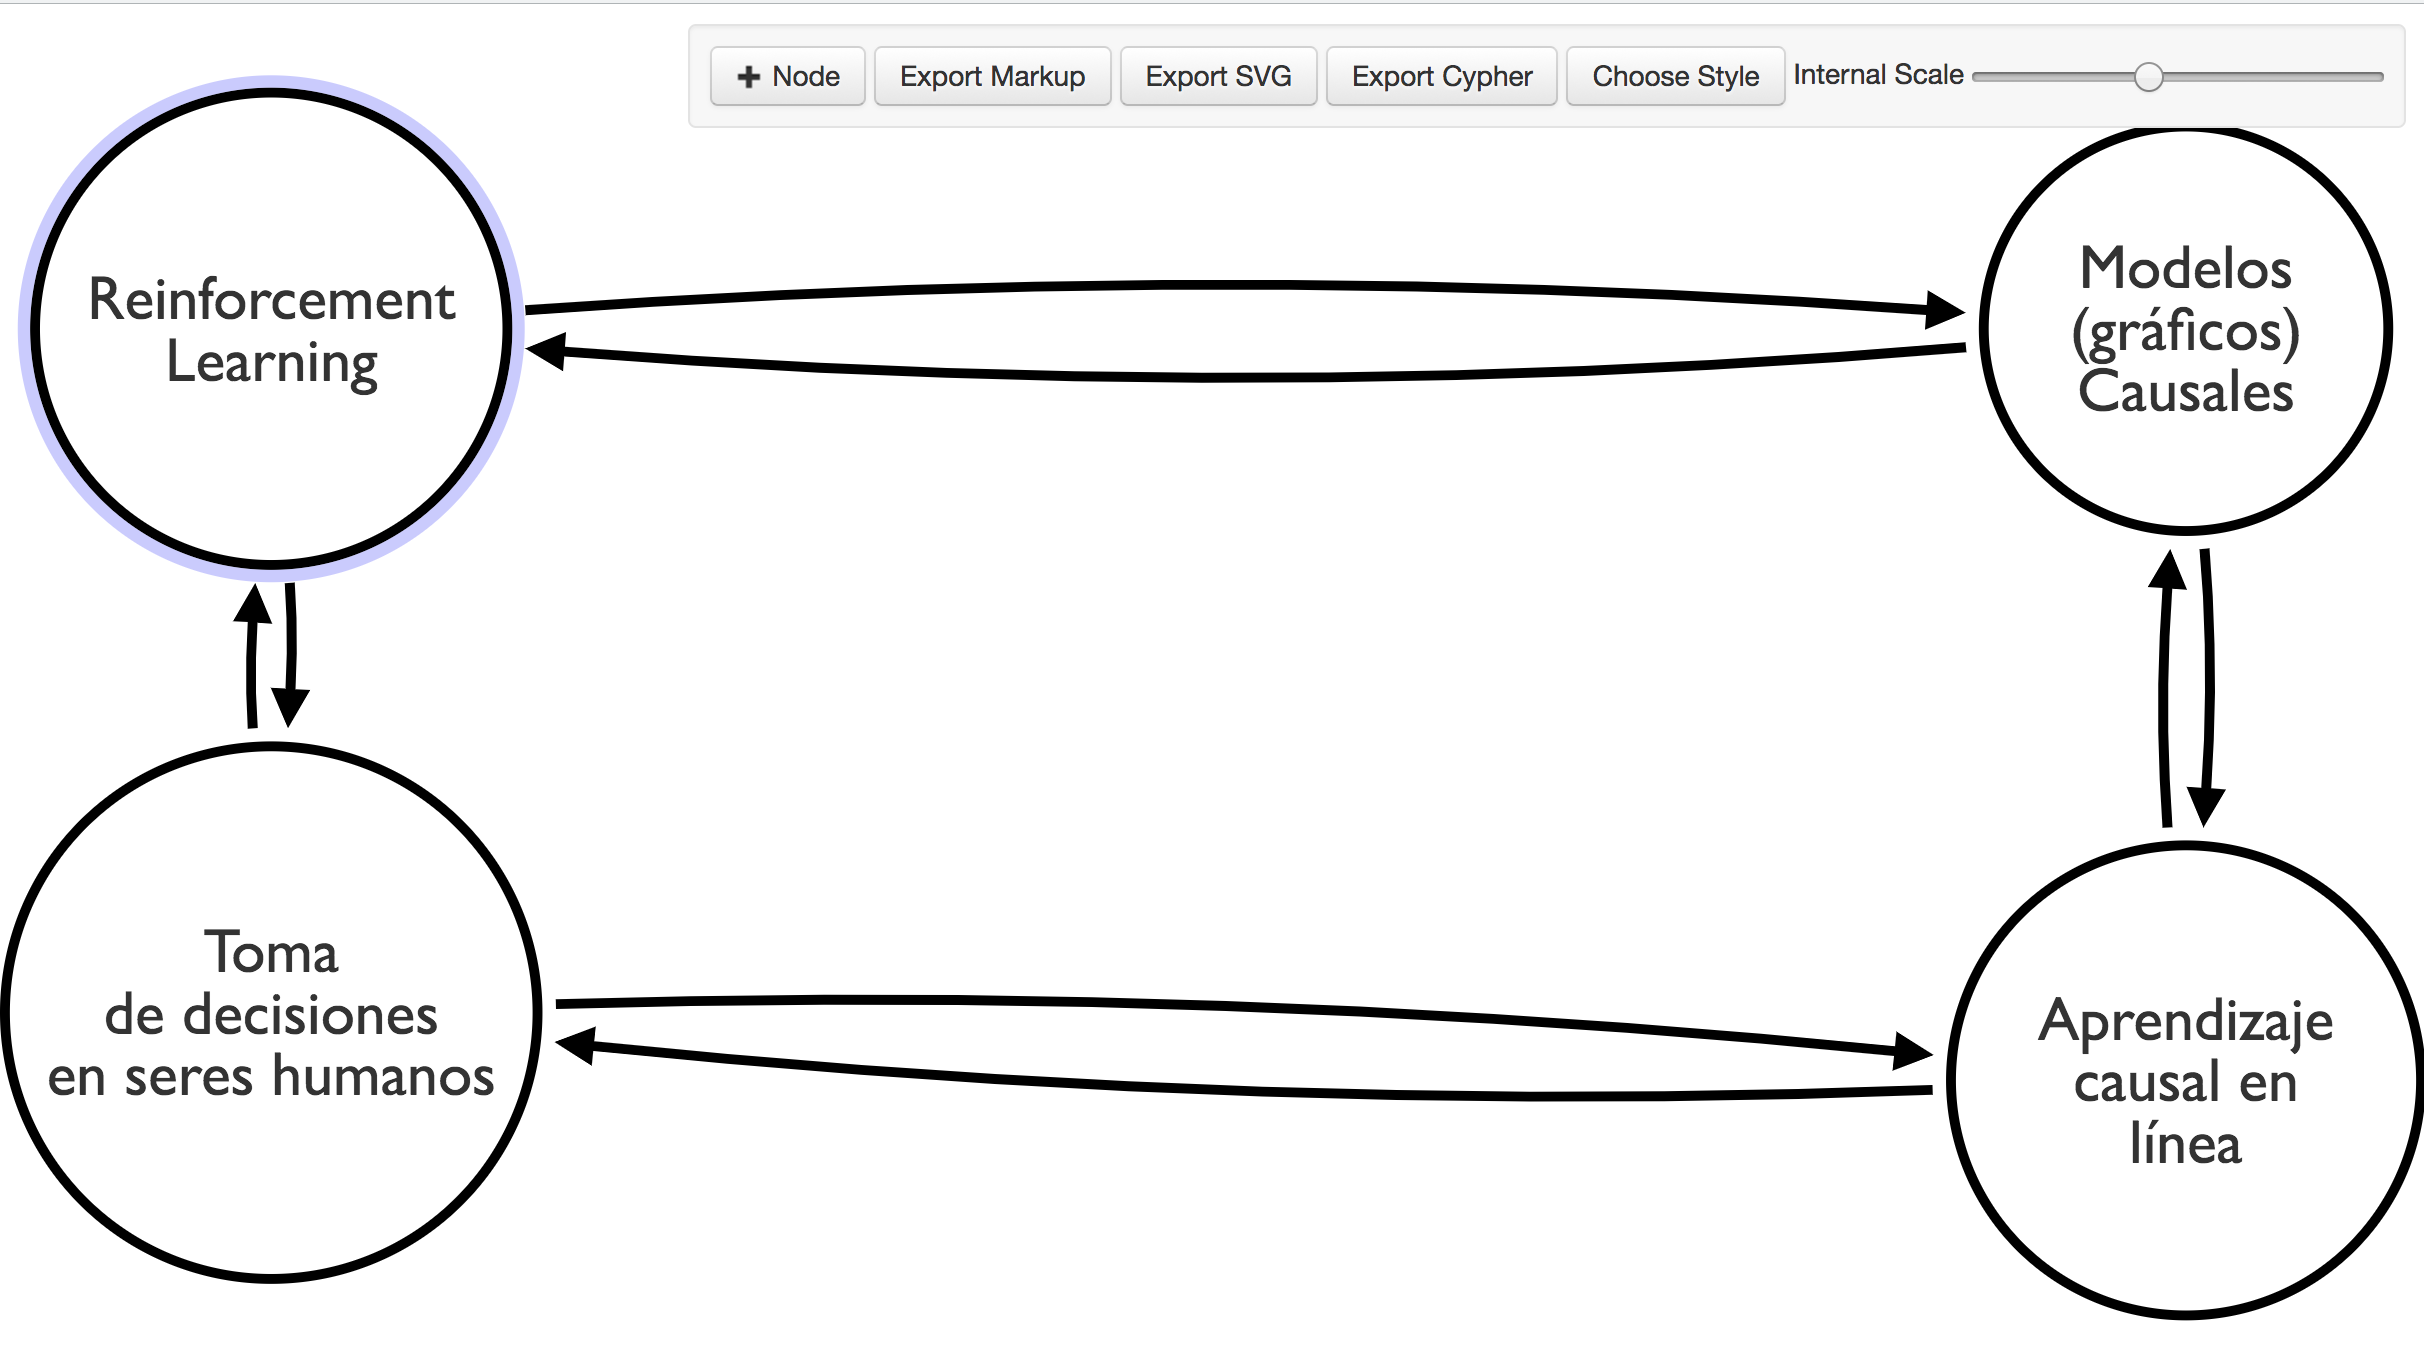
\includegraphics[scale=0.3]{/Users/MauricioGS1/INAOE/Primer_Semestre/Figures/diagrama.png}
\end{center}
\newpage
\bibliographystyle{apalike}
\bibliography{Bibliografia}
\end{document}